\documentclass[12pt,a4paper,oneside]{article}
%UPISATI JEZIK NA KOJEM JE NAPISAN RAD: HR ili EN
\def\jezik{HR}
\usepackage{lineno, blindtext}
\usepackage{gensymb}
\usepackage{subcaption}
\usepackage{graphicx}
\usepackage{float}
\usepackage{makecell}
\usepackage{amsmath}
\usepackage{spverbatim}
\usepackage{listings}
\usepackage{minted}


%UPIŠITE: DA ili NE
\def\dvostraniIspis{NE}

%POSTAVKE _setup.tex MORAJU BITI U ISTOJ MAPI GDJE JE I OVAJ DOKUMENT
%\usepackage{showframe} % pokaži marigine

% za brojanje
\usepackage[page,figure,table]{totalcount}

% prored: 1.5
\usepackage{setspace} 
\onehalfspacing

% omogućeni svi hr-znakovi
\usepackage[T1]{fontenc}
\usepackage[utf8]{inputenc}

% tekst-font: Times New Roman 12pt
\usepackage{times}
% promjena veličine fonta
\newcommand{\prored}[1]{\number\numexpr(#1*123)/100\relax}
\newcommand{\velicina}[2][22]{\fontfamily{ptm}\fontsize{#1 pt}{\prored{#1}pt}\selectfont#2}%\sffamily


% OSTALI POTREBNI PAKETI

%za pisanje formula
\usepackage{relsize}
\usepackage{amsmath,mathtools,amsfonts,amssymb,braket}
\usepackage{aurical,calrsfs} %kaligrafija \mathcal{}, \pazocal{}
\numberwithin{equation}{section}

%za liste
\usepackage{enumitem}

%za slike
\usepackage{graphicx,wrapfig,sidecap}
\usepackage[labelfont=bf,textfont={it},font=small]{caption}
\usepackage{pgf,tikz,pgfplots}
%\pgfplotsset{compat=1.11}
\usetikzlibrary{decorations.markings}
\usetikzlibrary{arrows,positioning,shadows}


% za tablice s više redova i definirane širine
\usepackage{multirow,array,colortbl,booktabs}
%\setlength\extrarowheight{3pt}
\newcommand{\urediTablicu}{\centering \fontsize{11pt}{17pt}\selectfont} % font 11pt, 17pt udaljene linije
\setlength{\arrayrulewidth}{0.75pt} % linije debljine 3/4 pt
\newcommand{\hlineRub}{\specialrule{1.5pt}{0pt}{0pt}} %debela horizontalna linija
\newcolumntype{?}{!{\vrule width 1.5pt}} %debela vertikalna linija



% float-naslovi
%\addtolength{\abovecaptionskip}{-3pt}
%\addtolength{\belowcaptionskip}{3pt}

%paketi koji omogućuju korištenje boja
\usepackage{color, xcolor}

%za isticanje i sakrivanje teksta
\usepackage{ulem}
\usepackage{comment}

%za pisanje veb adresa
\usepackage{url}
\urlstyle{same}
%\usepackage{hyperref} %otkomentirati za klikabilne linkove

%za lakšu usporedbu stilova
\usepackage{xstring}
\usepackage{ifthen}

% PRIJEVODI
%zamjena engleskih naziva s njihovim prijevodom
\ifthenelse{\equal{\jezik}{HR}}{
	\renewcommand\refname{\thesection~~~Literatura}
	%\renewcommand{\bibname}{Literatura}
	\renewcommand{\contentsname}{Sadr\v{z}aj}
	\renewcommand{\listfigurename}{Popis slika}
	\renewcommand{\listtablename}{Popis tablica}
	%\renewcommand{\abstractname}{Sa\v{z}etak}
	\renewcommand{\figurename}{Slika}
	\renewcommand{\tablename}{Tablica}
}{
	\renewcommand\refname{\thesection~~~Bibliography}
}

% POSTAVKE STRANICA

%zaglavlja
\usepackage{fancyhdr}
\fancyhf{} %uklanja defaultno zaglavlje/podnožje
\renewcommand{\headrulewidth}{0pt} % uklanja horizontalne crte
\fancyfoot[R]{\thepage}

% marigine
\usepackage[top=2.5cm, left=2.5cm, bottom=2.5cm, right=2.5cm]{geometry}

% dots in ToC
\usepackage{tocloft}
\renewcommand{\cftsecleader}{\cftdotfill{\cftdotsep}}

%uvlačenje paragrafa i razmak između
\setlength{\parindent}{0.4cm}
\setlength{\parskip}{6pt}


%POMOĆNE FUNKCIJE
%za računanje
\usepackage[nomessages]{fp}
\usepackage{calc}
%pomoći brojači za reference i stranice
\newcounter{brRef}\setcounter{brRef}{0}
\newcounter{brStr}\setcounter{brStr}{0}
%provjera postojanosti zahvale
\newlength{\duljinaZahvale}
%provjera postojanosti neposrednog voditelja
\newlength{\duljinaVoditelj}
\newlength{\dTabA}
\newlength{\dTabB}
%dijeljenje modulo
\newcommand{\modulo}[2]{%
	\FPeval{\rezModulo}{trunc(#1-(#2*trunc(#1/#2,0)),0)}%
}
\newcommand{\prijelom}[2]{%
	\ifthenelse{\equal{#1}{DA}\AND\equal{#2}{0}}%
	{~ \newpage}{}%
}
%vraća zadnju znamenku
\newcommand{\jed}[1]{\number\numexpr#1-10*((#1-5)/10)\relax}
%vraća zadnje dvije znamenke
\newcommand{\desJed}[1]{\number\numexpr#1-100*((#1-50)/100)\relax}
%sufiks za stranica, tablica, slika
\newcommand{\padez}[2]{%
	\ifthenelse{\equal{#2}{11}\OR\equal{#2}{12}\OR\equal{#2}{13}\OR\equal{#2}{14}}
		{a}%
		{\ifthenelse{\equal{#1}{2}\OR\equal{#1}{3}\OR\equal{#1}{4}}%
			{e}{\ifthenelse{\equal{#1}{1}}{u}{a}}}}
%sufiks za literaturni navod
\newcommand{\padezRef}[2]{%
	\ifthenelse{\equal{#1}{1}}%
		{literaturni navod}%
		{\ifthenelse{\equal{#2}{11}\OR\equal{#2}{12}\OR\equal{#2}{13}\OR\equal{#2}{14}}%
			{literaturnih navoda}%
			{\ifthenelse{\equal{#1}{2}\OR\equal{#1}{3}\OR\equal{#1}{4}}%
				{literaturna navoda}%
				{literaturnih navoda}}}}


% GENERATORI STRANICA
\newcommand{\kojiRad}{
	\ifthenelse{\equal{\vrstaRada}{1}}{
		\newcommand{\radHR}{Završni rad}
		\newcommand{\radEN}{Bachelor thesis}
	}{
		\newcommand{\radHR}{Diplomski rad}
		\newcommand{\radEN}{Master thesis}
	}
}

\newcommand{\naslovnica}{
	\pagestyle{empty} % bez br. str. 
	\kojiRad
	\begin{titlepage}
		\begin{center}
			\ifthenelse{\equal{\jezik}{HR}}{
				{\velicina[18]{Sveu\v{c}ili\v{s}te u Splitu\\
					Prirodoslovno – matemati\v{c}ki fakultet\\}}
				\vspace{\stretch{6}}
				{\velicina{\textbf{\naslovHR\\}}}
				\vspace{24pt}
				{\velicina[20]{\radHR\\}}
			}{
				{\velicina[18]{University of Split\\
					Faculty of Science\\}}
				\vspace{\stretch{6}}
				{\velicina{\textbf{\naslovEN\\}}}
				\vspace{24pt}
				{\velicina[20]{\radEN\\}}
			}
			\vspace{\stretch{4}}
			{\velicina{\student\\}}
			\vspace{\stretch{11}}
			{\velicina[14]{\mjestoVrijeme\\}}
		\end{center}
	\end{titlepage}
	\setcounter{brStr}{\arabic{page}}
	\stepcounter{brStr}
	\modulo{\thebrStr}{2}
	\prijelom{\dvostraniIspis}{\rezModulo}
	\pagestyle{fancy}
	\pagenumbering{roman}
}

\newcommand{\zahvale}{%
	\StrLen{\zahvala}[\duljinaZahvale]%duljina zahvale
	\ifthenelse{\equal{\duljinaZahvale}{0}}{}{
		\modulo{\arabic{page}}{2}
		\prijelom{\dvostraniIspis}{\rezModulo}
		\zahvala
		\newpage
		\modulo{\arabic{page}}{2}
		\prijelom{\dvostraniIspis}{\rezModulo}}{}
}

\newcommand{\stvoriTabove}{
	\StrLen{\neposredniVoditeljHR}[\duljinaVoditelj]
	\ifthenelse{\equal{\duljinaVoditelj}{0}}{
		\setlength{\dTabA}{3.0cm}
		\setlength{\dTabB}{12.7cm}
	}{
		\setlength{\dTabA}{3.5cm}
		\setlength{\dTabB}{12.2cm}
	}
}

\newcommand{\tdkHR}{
	\modulo{\arabic{page}}{2}
	\prijelom{\dvostraniIspis}{\rezModulo}
	\noindent
	\begin{tabular}{@{}l r@{}}
		\hline
		\multicolumn{2}{|@{}p{\textwidth}@{}|}{\centering \textbf{Temeljna dokumentacijska kartica}}\\
		\hline
		{}                    &  \\[-11pt]
		Sveu\v{c}ili\v{s}te u Splitu             & \radHR\\[-3pt]
		Prirodoslovno – matemati\v{c}ki fakultet &  \\[-3pt]
		Odjel za fiziku                          &  \\[-3pt]
		Ru\dj{}era Bo\v{s}kovi\'{c}a 33, 21000 Split, Hrvatska &  \\
	\end{tabular}
	\begin{center}
		{\velicina[11]{
			\textbf{\naslovHR}\\[12pt]
			\student\\[12pt]
			\studijHR\\[12pt]
		}}
	\end{center}
	\noindent \textbf{Sa\v{z}etak}:\\
	{\velicina[11]{\noindent\sazetakHR}}
	\stvoriTabove
	{\velicina[11]\begin{tabbing}
		\hspace{\dTabA}\=\hspace{\dTabB}\\[-12pt]
		\textbf{Klju\v{c}ne rije\v{c}i}: \> \kljucneRijeciHR\\[6pt]
		\textbf{Rad sadr\v{z}i}: \> \parbox[t][][t]{\dTabB}{
			\totalpages~stranic\padez{\jed{\totalpages}}{\desJed{\totalpages}}, 
			\totalfigures~slik\padez{\jed{\totalfigures}}{\desJed{\totalfigures}}, 
			\totaltables~tablic\padez{\jed{\totaltables}}{\desJed{\totaltables}}, 
			\thebrRef~\padezRef{\jed{\thebrRef}}{\desJed{\thebrRef}}.
			Izvornik je na \ifthenelse{\equal{\jezik}{HR}}{hrvatskom}{engleskom} jeziku.}\\[6pt]
		\textbf{Mentor}: \> \parbox[t][][t]{\dTabB}{\linespread{2} \mentorHR}
		\ifthenelse{\equal{\duljinaVoditelj}{0}}{\\[6pt]}{\\[6pt]\textbf{Neposredni voditelj}: \> \parbox[t][][t]{\dTabB}{\linespread{2} \neposredniVoditeljHR}\\[6pt]}
		\textbf{Ocjenjivači}: \> \parbox[t][][t]{\dTabB}{\linespread{2} \povjerenstvoHR}\\[6pt]
		\textbf{Rad prihvaćen}: \> \datumPrihvacanja 
	\end{tabbing}}
	{\velicina[11]{\noindent
		Rad je pohranjen u Knji\v{z}nici Prirodoslovno – matemati\v{c}kog fakulteta, Sveučilišta u Splitu.}}
	\newpage
	\modulo{\arabic{page}}{2}
	\prijelom{\dvostraniIspis}{\rezModulo}
}

\newcommand{\tdkEN}{
	\modulo{\arabic{page}}{2}
	\prijelom{\dvostraniIspis}{\rezModulo}
	\noindent
	\begin{tabular}{@{}l r@{}}
		\hline
		\multicolumn{2}{|@{}p{\textwidth}@{}|}{\centering \textbf{Basic documentation card}}\\
		\hline
		{}                    &  \\[-11pt]
		University of Split   &  \radEN\\[-3pt]
		Faculty of Science    &  \\[-3pt]
		Department of Physics &  \\[-3pt]
		Ru\dj{}era Bo\v{s}kovi\'{c}a 33, 21000 Split, Croatia & \\
	\end{tabular}
	\begin{center}
		{\velicina[11]{
			\textbf{\naslovEN}\\[12pt]
			\student\\[12pt]
			\studijEN\\[12pt]
		}}
	\end{center}
	\noindent \textbf{Abstract}:\\
	{\velicina[11]{\noindent\sazetakEN}}
	\stvoriTabove
	{\velicina[11]\begin{tabbing}
		\hspace{\dTabA}\=\hspace{\dTabB}\\[-12pt]
		\textbf{Keywords}: \> \kljucneRijeciEN\\[6pt]
		\textbf{Thesis consists of}: \> \parbox[t][][t]{\dTabB}{
			\totalpages~pages, \totalfigures~figures, \totaltables~tables, 
		\thebrRef~references. 
		Original language: \ifthenelse{\equal{\jezik}{HR}}{Croatian}{English}.}\\[6pt]
		\textbf{Supervisor}: \> \parbox[t][][t]{\dTabB}{\linespread{2} \mentorEN}
		\ifthenelse{\equal{\duljinaVoditelj}{0}}{\\[6pt]}{\\[6pt]\textbf{Leader}: \> \parbox[t][][t]{\dTabB}{\linespread{2} \neposredniVoditeljEN}\\[6pt]}
		\textbf{Reviewers}: \> \parbox[t][][t]{\dTabB}{\linespread{2} \povjerenstvoEN}\\[6pt]
		\textbf{Thesis accepted}: \> \datumPrihvacanjaEN 
	\end{tabbing}}
	{\velicina[11]{\noindent
		Thesis is deposited in the library of the Faculty of Science, University of Split.}}
	\newpage
	\modulo{\arabic{page}}{2}
	\prijelom{\dvostraniIspis}{\rezModulo}
}


\newcommand{\pocetak}{
	\newpage
	%početak teksta na neparnoj stranici
	\modulo{\arabic{page}}{2}
	\prijelom{\dvostraniIspis}{\rezModulo}
	% horizontalna crta zaglavlja
	\renewcommand{\headrulewidth}{0.75pt}
	\fancyhead[L]{\student: \kratkiNaslov}
	% horizontalna crta zaglavlja
	\pagenumbering{arabic}
}

% VARIJABLE ZA OSNOVNE INFORMACIJE
\def\student{}
\def\naslovHR{}
\def\naslovEN{}
\def\kratkiNaslov{}
\def\vrstaRada{}
\def\mjestoVrijeme{}
\def\zahvala{}
\def\studijHR{}
\def\studijEN{}
\def\sazetakHR{}
\def\sazetakEN{}
\def\kljucneRijeciHR{}
\def\kljucneRijeciEN{}
\def\mentorHR{}
\def\mentorEN{}
\def\povjerenstvoHR{}
\def\povjerenstvoEN{}
\def\datumPrihvacanja{}
\def\datumPrihvacanjaEN{}
\def\neposredniVoditelj{}
\def\neposredniVoditeljEN{}


% NOVE NAREDBE ZA PISANJE FORMULA
\newcommand{\vek}[1]{\vec{#1}}
\newcommand{\dif}{\mathrm{d}}
\newcommand{\ena}[1]{\exp\left(#1\right)}
\newcommand{\angstrem}{\textup{ \AA{}}}
\newcommand{\ddelta}[1]{\delta\left(#1\right)}
 

%POČETNE STRANICE SE GENERIRAJU AUTOMATSKI
% PRILAGODITE SAMO SADRŽAJ UNUTAR ZADNJIH {VITIČASTIH ZAGRADA} POJEDINE NAREDBE U NASTAVKU DO \begin{document}

\def\student{Leo Ivas}

\def\naslovHR{Mjerenje mase Higgsovog bozona u kanalu raspada na četiri miona s CMS eksperimentom u LHC-u}

\def\naslovEN{Higgs boson mass measurement in four muon decay channel with CMS experiment in LHC}

\def\kratkiNaslov{Mjerenje mase Higgsovog bozona u kanalu raspada na četiri miona s CMS eksperimentom u LHC-u}

% UPISATI 1 ili 2, 1 = završni rad, 2 = diplomski rad
\def\vrstaRada{2}

\def\mjestoVrijeme{Split, rujan 2020.}

\def\zahvala{Od srca se zahvaljujem svom dragom mentoru doc. dr. sc. Toniju Šćulcu na nesebičnom zalaganju,
	stručnom pristupu i prenesenom znanju pri izradi ovog diplomskog rada i studiranja.
	Hvala mojoj dragoj obitelji na bezuvjetnom razumijevanju i podršci tijekom mog akademskog obrazovanja.
	Hvala mojoj Katarini na bezgraničnoj podršci, poticajnosti i strpljenju.
	Hvala svim dobrim i dragim prijateljima.}

%IZBRISATI SVE DIJELOVE KOJI SE ODNOSE NA OSTALE STUDIJE
\def\studijHR{%
	Sveučilišni diplomski studij Fizika, Računarska fizika
}

\def\studijEN{%
	
	University graduate study programme Physics, Computational Physics
	}

\def\sazetakHR{
	U ovom diplomskom radu napravljen je pregled teorije standardnog modela u kojem smo pobliže opisali njegovu strukturu, a potom i objasnili ulogu elementarnih čestica. Potom smo dali matematički opis teorije preko grupa simetrije i opisali međudjelovanje jake, slabe i elektromagnetske sile preko baždarnih Lagrangiana. U kratkim crtama smo opisali osnovne mehanizme nastanka i raspada Higgsovog bozona od kojih smo neke koristili u daljnjoj analizi. Dotakli smo se i samog CERN-a i LHC-a, te opisali osnovne algoritme rekonstrukcije raspadnutih čestica, čije produkte možemo detektirati. Kako teorija SM-a ne predviđa masu Higgsovog bozona, morali smo se koristiti statističkom analizom obrade podataka kako bi iščitali istu. Za najpribližnije određivanje prave vrijednosti mase  Higgsovog bozona koristili smo se maximum likelihood metodom, a alat koji nam je pomogao u prilagođavanju podataka na funkciju i grafičko prezentiranje rezultata je bio programski paket RooFit. Prema teoriji SM-a konstruirali smo double Crystal ball funkciju, koja se u konačnici pokazala jako dobro prilikom uspoređivanja s pravim podatcima. Konačni dobiveni rezultat za masu Higgsovog bozona je m${_{\mathrm{H}}^{4\mu}}$ = 124,96 $\pm$ 0,17(stat.)$_{-0,28}^{+0,27}$(sist.) GeV, a usporedbom tog rezultata s onima iz CERN-a vidimo slaganje unutar pogreške.}

\def\sazetakEN{
	In this thesis, an overview of the theory of the standard model is made, in which we describe its structure in more detail, and then explain the role of elementary particles. We then gave a mathematical description of the theory with symmetry groups and described the interaction of strong, weak, and electromagnetic forces with Lagrangians. We have briefly described the basic mechanisms of the formation and decay of the Higgs boson, some of which we use in further analysis. We also mentioned CERN and the LHC, and described the basic algorithms for the reconstruction of decayed particles, whose products we can detect. Since SM theory does not predict the mass of the Higgs boson, we had to use statistical analysis of data processing to read the same. To most closely determine the true value of the mass of the Higgs boson, we used the maximum likelihood method, and the tool that helped us fit the data to the function and graphically present the results was the RooFit software package. According to SM theory, we constructed a double Crystal ball function, which ultimately proved very good when compared to real data. The final result obtained for the mass of the Higgs boson is m ${_{\mathrm {H}}^{4 \mu}}$ = 124,96 $ \pm $ 0,17 (stat.) $_{- 0,28}^{+ 0,27}$ (syst.) GeV, and by comparing this result with those from CERN we see agreement within the error.}


\def\kljucneRijeciHR{Higgsov bozon, CERN, LHC, CMS, double Crystal ball }

\def\kljucneRijeciEN{Higgs boson, CERN, LHC, CMS, double Crystall ball}

% AKO POSTOJI VIŠE MENTORA, DODAJTE IH SLIČNO KAO ČLANOVE POVJERENSTVA (POGLEDAJTE U NASTAVKU)

% OSTAVITE SAMO JEDNU OD TITULA prof. ili izv. prof. ili doc.
\def\mentorHR{{doc.} dr. sc. Toni Šćulac}

% OSTAVITE SAMO JEDNU OD TITULA Prof. ili Asoc. Prof. ili Assist. Prof.
\def\mentorEN{{Assist. Prof.} Dr. Toni Šćulac}

% AKO NE POSTOJI NEPOSREDNI VODTELJ, IZBRISITE TEKST UNUTAR VANJSKIH VITICASTIH ZAGRADA
% AKO POSTOJI NEPOSREDNI VODTELJ, OSTAVITE SAMO JEDNU ILI NIJEDNU OD TITULA prof., izv. prof. ili doc odnosno Prof. ili Asoc. Prof. ili Assist. Prof.
\def\neposredniVoditeljHR{}
\def\neposredniVoditeljEN{}

% ODVOJITE ČLANOVE SA ,\\ I OSTAVITE SAMO JEDNU ILI NIJEDNU TITULU U UNUTARNJIM ZAGRADAMA
\def\povjerenstvoHR{
	{doc.} dr. sc. Toni Šćulac,\\
	{doc.} dr. sc. Marko Kovač,\\
	{prof.} dr. sc. Ivica Puljak
}

% ODVOJITE ČLANOVE SA ,\\ I OSTAVITE SAMO JEDNU ILI NIJEDNU TITULU U UNUTARNJIM ZAGRADAMA
\def\povjerenstvoEN{
	{Assist. Prof.} Dr. Toni Šćulac,\\
	{Assist. Prof.} Dr. Marko Kovač,\\
	{Prof.} Dr. Ivica Puljak
}

\def\datumPrihvacanja{DAN. MJ. GOD.}
\def\datumPrihvacanjaEN{Month day, Year}


% UPISATI UKUPAN BROJ LITERATURNIH NAVODA UNUTAR ZADNJE ZAGRADE (nakon definiranja cjelokupne literature)
\setcounter{brRef}{7}


\begin{document}
	\naslovnica % stvara naslovnu stranicu
	\zahvale % ispisuje zahvale ako postoje
	\tdkHR \tdkEN % stvara temeljne dokumentacijske kartice
	\tableofcontents %popis naslova
	%\newpage\listoffigures % ukloniti % na početku linije za popis slika
	%\newpage\listoftables  % ukloniti % na početku linije za popis tablica
	\pocetak %postavke zaglavlja, uvod na neparnoj stranici
	

	% SVA POGLAVLJA RADA UNIJETI U NASTAVKU
	\begin{linenumbers}
		\section{Uvod}
		Glavna tema ovog diplomskog rada je mjerenje mase Higgsovog bozona u kanalu raspada Higgsovog bozona na 4 miona. To je jedan od najvažnijih kanala raspada koji predviđa teorija standardnog modela (SM) predložena 70-ih godina 20. stoljeća. Iako je SM i prije otkrića Higgsovog bozona jako dobro opisivano procese jakih, slabih i elektromagnetskih međudjelovanja, može se reći da je svoju potpunost doživio tek 4. srpnja 2012. godine kada su u CERN-u, CMS i ATLAS u kolaboraciji objavili otkriće nove čestice. 
		Nakon uvoda, u 2. poglavlju ćemo opisati matematičku postavku standardnog modela koja je bila i ključni kamen temeljac u izradi simulacija koje su od velike važnosti za dokazivanje same teorije.
		Kompleksni proces dokazivanja ovakve vrste teorije u čestičnoj fizici je detaljnije opisan u radu, no ugrubo se može podijeliti u 4 osnovna koraka: postavljanje teorije, izrada računalne simulacije prethodno postavljenog teoretskog modela, pronalaženje idealne matematičke funkcije koja najbolje opisuje takav model te provjeravanje vjerodostojnosti modela prilagođavanjem na prave izmjerene podatke.
		Podatci na kojima smo radili prikupljani su u periodu od 2015. do 2018. godine, a detaljan način stvaranja procesa i prikupljanja podataka opisan je u 3. poglavlju. 
		U 4. poglavlju smo objasnili statističku i računarsku pozadinu obrade ovakve vrste podataka, dok smo u 5. poglavlju prezentirali konačne rezultate i usporedili ih s onima iz CERN-a objavljenim u prethodnom ciklusu prikupljanja podataka.
		
		\newpage
		\section{Teorijski uvod}
		
		\subsection{Standardni model}
		
		Standardni model (SM) elementarnih čestica je teorija koja opisuje elektroslabo i jako međudjelovanje čestica~\cite{uvod}. Unatoč tome što ne sadrži opis gravitacijskog međudjelovanja, trenutno je najbolja teorija koja opisuje međudjelovanje elementarnih čestica.
		Elementarne čestice u SM-u podijeljene su u dvije osnovne skupine: fermioni i bozoni.
		\begin{figure}[H]
			\centering
			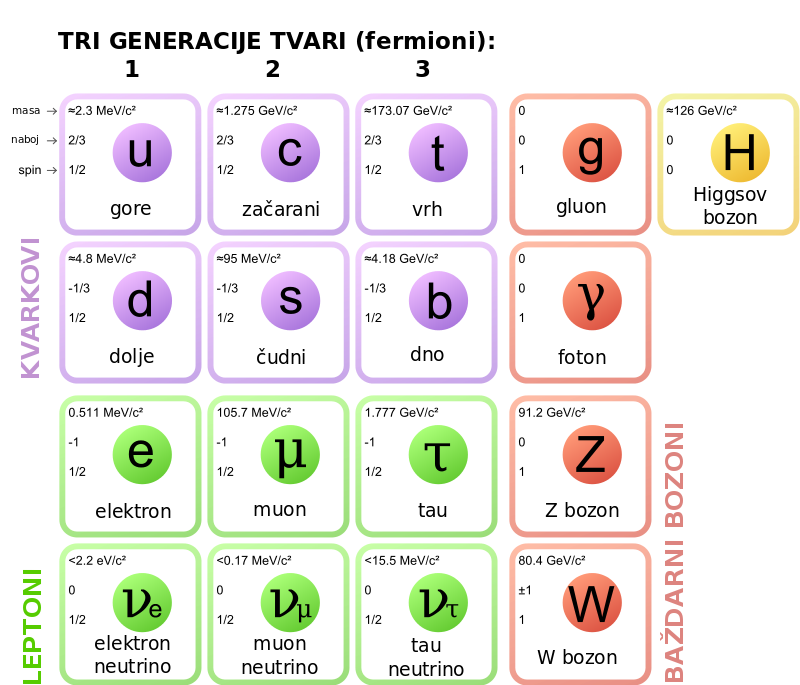
\includegraphics[width=0.8\textwidth]{Standard_Model_of_Elementary_Particles_hr.png}
			\caption[SM]{\label{sl:primjer}Tablica elementarnih čestica u standardnom modelu ~\cite{standardni_model}.}
		\end{figure}
		
		
		\subsubsection{Fermioni}
		Fermioni su čestice spina 1/2 koje izgrađuju materiju i dijelimo ih u dvije podskupine: kvarkove i leptone, a svaku od podskupina možemo podijeliti u tri generacije. Svaki element veće generacije ima veću masu s izuzetkom neutrina čija masa još nije točno izmjerena.
		\paragraph{Kvarkovi\newline}
		
		Do otkrića kvarkova, fizičari su znali samo za električni naboj koji je cjelobrojni višekratnik elementarnog naboja te se smatralo da je kvant elementarnog naboja jednak naboju elektrona. Sada vjerujemo da je kvant  jednak naboju kvarka~\cite{uvod2}. Ipak, zbog povijesnih razloga ostali smo pri staroj notaciji pa tako elektron ima električni naboj -e, proton +e, jezgra helija +2e i tako dalje. Kvarkovi, ovisno o vrsti, imaju samo dio elementarnog naboj: $+\frac{2}{3}$e ili $-\frac{1}{3}$e. Budući da kvarkovi ne postoje samostalno već uvijek dolaze u kombinaciji dva ili tri kvarka, u prirodi nije moguće zapaziti čestice s nabojem manjim od jednog elementarnog naboja. Čestice sastavljene od tri kvarka nazivamo barionima, dok mezonima nazivamo čestice sastavljene od para kvarka i antikvarka. Sva materija u svemiru sastoji se od atoma, dakle od protona i neutrona, stoga su gornji i donji kvarkovi najviše zastupljeni kvarkovi u svemiru. Ostali kvarkovi su puno masivniji (masa kvarkova raste kako idemo od prve prema drugoj i trećoj generaciji) i puno rjeđi. Međutim, ranije u evoluciji svemira tvar je bila daleko energičnija, stoga su masivniji kvarkovi bili mnogo češći i imali su značajniju ulogu u reakcijama koje su se tada događale.
		
		\paragraph{Leptoni\newline}
		Od leptona najpoznatiji je elektron, stoga su leptoni najviše i proučavani budući da se svojstva elektrona zrcale u mionu i tau leptonu~\cite{uvod2}. Navedena tri leptona imaju isti električni naboj i osim mase, malo toga razlikuje elektron od miona i tau leptona. Jedina očita razlika je u tome što se mion i tau lepton mogu raspadati na druge čestice (iz prve i druge generacije leptona i njihove antičestice), dok je elektron stabilna čestica. Isto kao i kod kvarkova, masa leptona se povećava kako idemo prema višoj generaciji.
		Ostala tri leptona se nazivaju neutrini jer su električki neutralni.
		Leptoni, za razliku od kvarkova, postoje u prirodi kao zasebne čestice. 
		Leptoni druge generacije su rjeđi, ali ih se može naći u prirodi. Mione je lako proizvesti u laboratorijskim pokusima i osim po masi, vrlo su slični elektronima. Zbog velike mase su nestabilni pa se raspadaju na elektrone i neutrina. Članovi treće generacije nisu viđeni u nikakvim prirodnim procesima, barem ne u ovom stadiju evolucije svemira. Mnogo ranije, kada je svemir bio topliji i kada su čestice imale daleko više energije, leptoni treće generacije su često nastajali u prirodnim reakcijama. Danas se tau lepton može promatrati samo u laboratorijskim pokusima, dok tau neutrino nije izravno viđen u pokusima već se njegovo prisustvo daje zaključiti indirektno mjerenjem energije iz određenih reakcija.
		
		\subsubsection{Bozoni}
		Za razliku od fermiona koji izgrađuju materiju, bozoni su čestice međudjelovanja i njihov spin je cjelobrojan. Skupini baždarnih bozona spina 1, pripadaju fotoni, gluoni, W-bozoni i Z-bozoni, dok Higgsov bozon spada u skalarne bozone i njegov spin je 0.
		
		\paragraph{Fotoni\newline}
		Foton je osnovni djelić energije elektromagnetskog zračenja i on je elementarna čestica koja je posrednik u prenošenju elektromagnetskog međudjelovanja~\cite{uvod3}. U vakuumu se foton giba brzinom svjetlosti te nema masu, električni naboj, niti energiju mirovanja.
		\paragraph{W i Z bozoni\newline}
		$\rm{W}^{\pm}$ i Z bozoni su elementarne čestice prijenosnici slabe nuklearne sile, odgovorne za raspade protona u neutrone i obrnuto~\cite{uvod4}. Za razliku od ostalih baždarnih bozona, mase mirovanja su im različite od nule, a iznose 80,4 i 91,2 GeV/c$^2$, što je gotovo 100 puta veće od mase protona, zbog čega im je djelovanje ograničeno na atomsku jezgru.
		\paragraph{Gluoni\newline}
		Gluon  je elementarna čestica bez mase, koja prenosi jako međudjelovanje i veže kvarkove u hadrone~\cite{uvod5}. Međudjelovanje kvarkova prenosi se emisijom i apsorpcijom gluona, slično kao što se elektromagnetsko međudjelovanje prenosi fotonima. 
		
		
		Valja naglasiti da i svaka čestica ima svoju antičesticu suprotnog kvantnog broja i najčešće joj simbol isti kao čestica samo s povlakom (npr. mion $\mu$ , antimion \begin{math}
		\bar{\mu}
		\end{math}).
		
		
		\subsection{Lagrangian SM-a}
		SM teoretski možemo opisati objedinjenjem dvije teorije: kvantna elektrodinamika (eng. Quantum Electrodynamics, QED) i kvantna kromodinamika (eng. Quantum Chromodynamics, QCD). Sva tri međudjelovanja koja opisuje SM funkcioniraju u posredstvu nekog baždarnog bozona. Lagrangian SM-a je simetričan s obzirom na baždarnu grupu~\cite{doktorat}: 
		\begin{equation}
		SU(3) \otimes SU(2) \otimes U(1)
		\end{equation}
		QCD teorija opisuje jako međudjelovanje i bazirana je na \begin{math}
		SU(3)
		\end{math}  grupi, dok  QED objašnjava elektroslabo međudjelovanje i simetrična je \begin{math}
		SU(2) \otimes U(1)
		\end{math} grupi~\cite{doktorat}. 
		
		\subsubsection{Baždarna invarijantnost}
		Neka su električno i magnetsko polje opisani preko vektorskih i skalarnih potencijala na idući način~\cite{dokt2}:
		\begin{equation}
		\boldsymbol{E} = -\nabla \phi - \frac{\partial \boldsymbol{A}}{\partial t}
		\end{equation}
		\begin{equation}
		\boldsymbol{B} = \nabla \times \boldsymbol{A}
		\end{equation}
		Ako za potencijale vrijede baždarne transformacije~\cite{dokt2}:
		\begin{equation}
		\phi \rightarrow \phi + \frac{\partial \psi}{\partial t}
		\end{equation}
		\begin{equation}
		\boldsymbol{A} \rightarrow \boldsymbol{A} - \nabla \psi 
		\end{equation}
		to znači da električno i magnetsko polje nisu jedinstveno opisani, no baždarne transformacije su ih očuvale. Ako zapisujemo preko četverovektora potencijala i operatora diferencijala ,baždarna transformacija može se definirati kao:
		\begin{equation}
		A_\mu \rightarrow A_\mu ^{'} = A_\mu + \frac{1}{e} \partial_\mu \alpha
		\end{equation}
		gdje e označava električni naboj~\cite{dokt2}.
		
		\paragraph{Lagrangian elektromagnetskog međudjelovanja\newline} 
		Ako Maxwellovu jednadžbu za slobodno elektromagnetsko (EM) polje  zapišemo u Lorentz kovarijantnom obliku:
		\begin{equation}
		\partial_\mu F_{\mu v} = 0
		\end{equation}
		gdje je \begin{math}
		F_{\mu v} = \partial_\mu A_v - \partial_v A_\mu 
		\end{math}
		primjenjujući baždarne transformacije vidimo da tenzor jakosti EM polja ostaje nepromijenjen, stoga zaključujemo da je baždarno invarijantan što znači da su Maxwellove jednadžbe baždarno invarijantne~\cite{dokt2}. 
		Uvedimo sada Langrangian za slobodno elektromagnetsko polje:
		\begin{equation}
		L_{EM} = - \frac{1}{4} F_{\mu v} F_{v \mu}
		\end{equation}
		Baždarne tranfsormacije na tom Langrangianu se mogu opisati Abelovom grupom \begin{math}
		U(1)
		\end{math} . Kada govorimo o Abelovoj grupi mislimo na  matematički objekt linearne algebre čiji elementi zadovoljavaju svojstva: zatvorenosti, asocijativnosti, postojanje neutralnog elementa, postojanje inverznog elementa i komutativnosti.
		Ta grupa simetrije \begin{math}
		U(1)
		\end{math} ima jedan generator i to predstavlja postojanje jedne čestice medijatora elektromagnetne sile (fotona)~\cite{dokt2}.
		Ukupni baždarno invarijantni Langrangian za QED je dan kao: 
		\begin{equation}\
		L_{QED}= -\frac{1}{4} F_{\mu v} F_{v \mu} + \bar{\psi}x [i \gamma^\mu (\partial_\mu - i e A_\mu) -m]\psi(x)
		\end{equation}
		\paragraph{Lagrangian elektroslabog međudjelovanja\newline}
		
		Isti princip baždarne invarijantnosti koji vrijedi za QED može se primijeniti na elektroslabo međudjelovanje koje zapravo objedinjuje dvije teorije međudjelovanja elektromagnetsko i slabo nuklearno~\cite{doktorat}. Ono obuhvaća  \begin{math}
		U(1)
		\end{math} grupu koja opisuje EM međudjelovanja i \begin{math}
		SU(2)
		\end{math} grupu koja opisuje isospin slabog međudjelovanja. Grupa simetrije \begin{math}
		SU(2) \times U(1) 
		\end{math} ima 4 generatora što zapravo predstavlja 4 čestice medijatora, 3 za slabo međudjelovanje (\begin{math}
		W^+
		\end{math}, \begin{math}
		W^-
		\end{math} i \begin{math}
		Z
		\end{math} bozon), te jednu česticu za elektromagnetsko međudjelovanje (foton).
		
		Lagrangian elekroslabog međudjelovanja možemo zapisati kao~\cite{doktorat}:
		
		\begin{align}\label{eq:3}
		\begin{split}
		L_{EW} ={}& \bar{L}i\gamma^{\mu}\partial_\mu L + \bar{\psi '}_R i\gamma^{\mu}\partial_\mu \bar{\psi '}_R \\
		& - g_w \bar{L}\gamma^\mu \frac{\sigma_i}{2} L {W_\mu}^i - g \bar{L}\gamma^\mu \frac{Y}{2} L B_\mu - g \bar{{\psi'}_R}\gamma^\mu \frac{\sigma_i}{2} {\psi'}_R {B_\mu} \\ 
		&- \frac{1}{4}{W_{i}^{\mu v}} W_{\mu v}^{i} - \frac{1}{4}{B^{\mu v}} {B}_{\mu v}
		\end{split}
		\end{align}
		Kratki doseg slabe nuklearne sile nam ukazuje da čestice međudjelovanja moraju imati masu, a to implicira da simetrija koja stoji iza ove teorije ne funkcionira, tj. da postoji nekakav mehanizam koji daje masu česticama izmjenjenim u slabim međudjelovanjima (W i Z bozonima), ali ne daje masu česticama izmjenjenim u električnim međudjelovanjima (fotonima). Eksperimenti su pokazali nepobitne dokaze da slaba sila stvarno postoji sa svim svojim svojstivma i česticama, što je samo značilo da treba pronaći nešto što krši simetriju te teorije.
		
		\paragraph{Lagrangian jakog međudjelovanja\newline}
		Na sličan način kao i za elektroslabo međudjelovanje, grupa simetrije \begin{math}
		SU(3) 
		\end{math} ima 8 generatora tj. 8 čestica međudjelovanja u jakoj nuklearnoj sili (gluoni)~\cite{doktorat}. Langrangian takvog međudjelovanja dan je sa:
		\begin{equation}\label{eq:2}
		\begin{split}
		L_{QCD} = \bar{\psi_i}(i{(\gamma^\mu D_\mu)}_{ij} - m\delta_{ij})\psi_j - \frac{1}{4} G^a_{\mu v}G^{\mu v}_a 
		\end{split}
		\end{equation}
		
		
		
		\subsubsection{Spontano narušenje simetrije}
		Problem koji smo naveli u prošlom odlomku je vrlo elegantno riješen s tzv. BEH (Brout-Englert-Higgs) mehanizmom. To je zapravo mehanizam koji $\rm{W}^{\pm}$ i Z bozonima daje masu kada međudjeluju s nevidljivim poljem koje nazivamo Higgsovo polje~\cite{cernweb}. Odmah nakon velikog praska iznos Higgsovog polje je bilo 0, no kako se svemir hladio i temperatura pala ispod kritične vrijednosti, polje je spontano raslo i kao posljedica toga u međudjelovanju s česticama davalo im masu. Kada se to ne bi događalo, ne bi ni bilo moguće razlučiti između 3 generacije elementarnih čestica jer po svim ostalim svojstvima su jednaki osim po masi. Što više čestica međudjeluje s poljem to teža postaje. Čestice poput fotona ne međudjeluju s poljem stoga ni nemaju masu.
		Sam koncept Higgsovog mehanizma je veoma sličan efektu feromagnetizma u kojem zbog jakog međudjelovanja magnetskih momenata atoma dolazi do kolektivnog magnetskog uređenja tzv. spontane magnetizacije. U  vanjskom magnetskom polju, feromagnetične tvari postaju inducirani magneti koje zatim to polje privlači.  
		Naravno intuitivno je jasno i da za Higgsovo polje postoji čestica Higgsov bozon koji možemo zamisliti kao nekakvu pobudu u polju, kao npr. val na površini mora~\cite{cernweb}. 
		
		\paragraph{Lagrangian Higgsovog polja\newline}
		Lagrangian koji opisuje Higgsovo polje zadan je kao~\cite{doktorat}:
		\begin{align}\label{eq:4}
		\begin{split}
		L_{Higgs} ={}& \frac{1}{2} \partial_\mu h \partial^\mu h + \mu^2 h^2 \\ &+ \frac{g_w^2 v^2}{4} {W_{\mu}^{-}} {W^{+\mu}} + \frac{g^2_w v^2}{8 \cos^2 \theta_w} Z_\mu Z^\mu \\ &+ \frac{g^2_w v^2}{2} h {W_{\mu}^{-}} {W^{+\mu}} + \frac{g^2_w }{4} h^2 {W_{\mu}^{-}} {W^{+\mu}} + \frac{g^2_w v}{4 \cos^2 \theta_w} h {Z}_\mu {Z^{\mu}} + \frac{g^2_w}{8 \cos^2 \theta_w} h^2 {Z}_\mu {Z^{\mu}} \\ &+ \frac{\mu^2}{v} h^3 + \frac{\mu^2}{4v^2} h^4
		\end{split}
		\end{align}
		Važno je naglasiti da je masa Higgsovog bozona (\begin{math}
		m_H = \sqrt{|\mu|}
		\end{math})  slobodan parametar koji se ne može odrediti direktno iz teorije, već se mora izmjeriti.
		Također, BEH mehanizam se iskoristio i za proširenje SM-a s baždarno invarijantnim Yukavinim članom koji je zadužen za davanje mase fermionima. On je zadan kao:
		\begin{equation}\label{eq:5}
			L_{Yukawa} = \sum_{f} -m_f \bar{\psi} \psi (1 + \frac{h}{v}) + \sum_{f'} -m_f \bar{\psi'} \psi' (1 + \frac{h}{v})
		\end{equation} 
		gdje prva suma ide po gornjem tipu fermiona, a druga po donjem tipu fermiona.
		
		Konačni Lagrangian SM-a možemo pisati kao sumu jednadžbi \ref{eq:2}, \ref{eq:3}, \ref{eq:4} i \ref{eq:5} ~\cite{doktorat}:
		\begin{equation}
			L_{SM} = L_{QCD} + L_{EW} + L_{Higgs} + L_{Yukawa}
		\end{equation}
		
		
		\subsection{Higgsov bozon}
		Teoretski model koji smo opisali u prošlom poglavlju  je predložen još 70-ih godina prošlog stoljeća, no eksperimentalno je dokazan tek 2012. godine. Te godine, 4. srpnja, CMS i ATLAS eksperiment su  objavili nepobitne dokaze o posljednjem velikom koraku koji je upotpunio SM kojeg poznajemo i dan danas~\cite{doktorat}. Nakon izbacivanja prvih  rezultata, znanstvenici iz europske organizacije za nuklearna istraživanja (fra. Conseil Européen pour la Recherche Nucléaire, CERN)  nastavili su nadograđivati Veliki Hadronski Sudarač (eng. Large hadron colider, LHC) te su dobivali sve pouzdanije i točnije rezultate. Najbolji primjer koliko se eksperiment razvio prikazuje slika \ref{sl:luminozitet}  koja pokazuje  porast luminoziteta  tijekom godina istraživanja, odnosno koliko se sudara dogodi u akceleratoru.
		
			\begin{figure}[H]
			\centering
			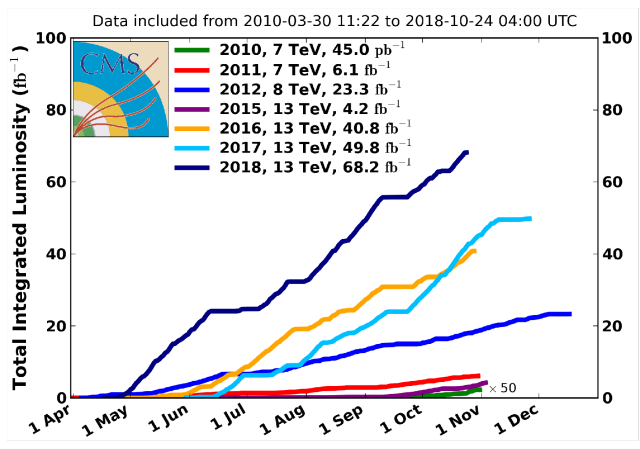
\includegraphics[width=0.8\textwidth]{luminozitet.png}
			\caption[Vremenska evolucija ukupnog integriranog luminoziteta podataka prikupljenih s CMS eksperimentom za različite godine djelovanja.~\cite{doktorat}]{\label{sl:luminozitet}Vremenska evolucija ukupnog integriranog luminoziteta podataka prikupljenih s CMS eksperimentom za različite godine djelovanja~\cite{doktorat}. }
		\end{figure}
		\subsubsection{Mehanizam proizvodnje Higgsovog bozona}
		Govoreći o SM-u neizbježno je spomenuti i Feynmanove dijagrame. To su grafičke ilustracije matematičkih izraza koje opisuju ponašanje i međudjelovanje elementarnih čestica, a uveo ih je američki fizičar Richard Phillips Feynman 50-ih godina 20. stoljeća. Oni će nam pomoći pri opisu glavnih mehanizama proizvodnje tj. nastajanja Higgsovog bozona. Iako postoji više načina za nastajanje Higgsova bozona mi ćemo se koncentrirati samo na one koji su najvažniji u LHC-u ~\cite{doktorat}.
		
		\paragraph{Fuzija gluona\newline}
		Fuzija gluona je proces u kojem se dva gluona udružuju u međukoraknu petlju kvarkova, a potom iz te petlje nastaje Higgsov bozon~\cite{doktorat}. Taj proces se događa najčešće u oko 89\% slučajeva, što je pokazano najvećim udarnim presjekom od svih ostalih načina proizvodnje. Razlog tome leži u činjenici da je luminozitet gluona jako velik u proton-proton sudarima visoke energije koje LHC može proizvesti.
		\begin{figure}[H]
			\centering
			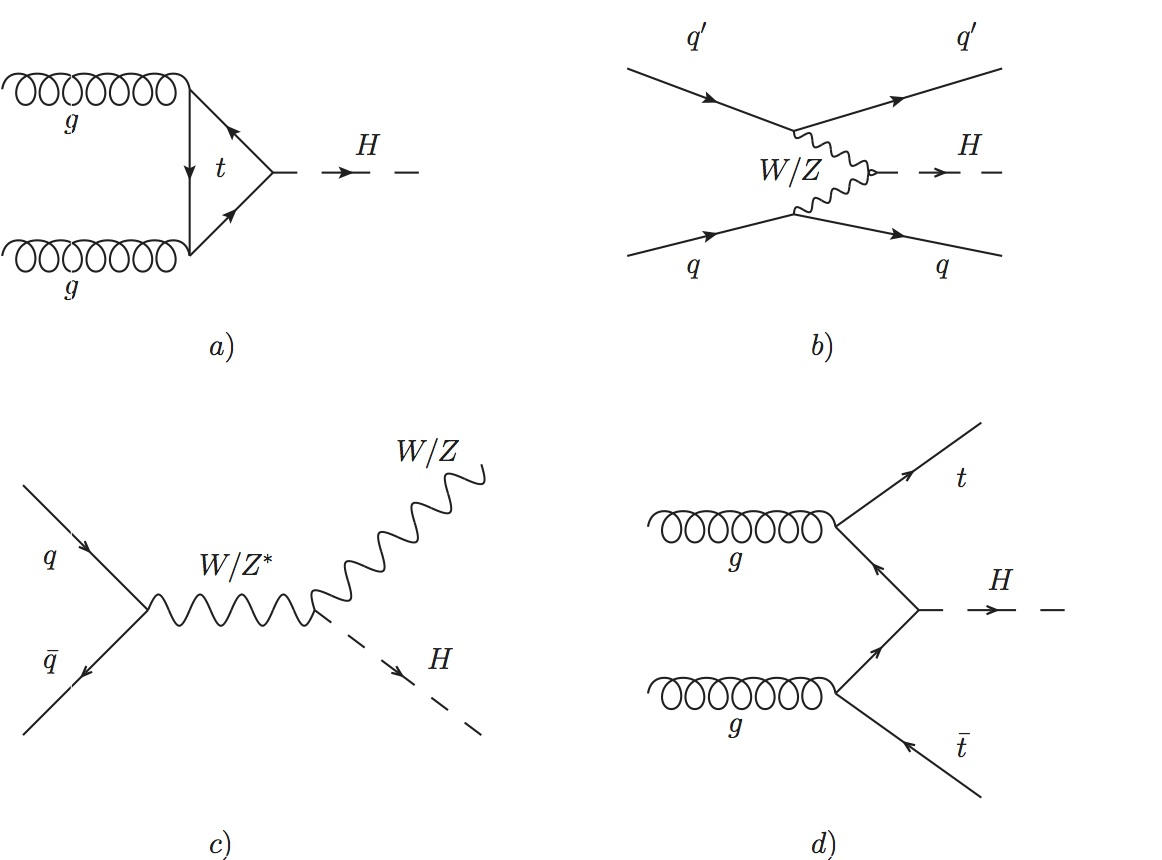
\includegraphics[width=0.8\textwidth]{higgs-production.jpg}
			\caption[Saturn viđen u  svjetlu.]{\label{sl:gluon-fuzija}a) Fuzija gluona, b)Fuzija vektorskih bozona, c)Procesi s pridruženom proizvodnjom W ili Z bozona, d)Procesi s pridruženom proizvodnjom \begin{math}
				t \bar{t}
				\end{math}  para  ~\cite{doktorat}. }
		\end{figure}
		
		\paragraph{Ostali načini proizvodnje\newline}
		Fuzija vektorskih bozona je drugi najčešći način proizvodnje Higgsovog bozona, ali udarni presjek tog procesa je manji za čak jedan red veličine od gluon gluon fuzije~\cite{doktorat}. Ovaj proces se događa kada dva fermiona izmjene virtualne W ili Z bozone koji se trenutno udružuju i prelaze u Higgsov bozon.
	
		Procesi s pridruženom proizvodnjom W ili Z bozona su treći najučestaliji način proizvodnje Higgsovog bozona. U tom procesu se fermion i antifermion sudare i proizvedu W ili Z bozon koji nakon toga izrači Higgsov bozon. Kao izlaz u tom procesu vidimo Higgsov bozon koji je popraćen sa leptonskim ili hadronskim česticama koji su proizvod  W ili Z bozona.
		
		Procesi s pridruženom proizvodnjom \begin{math}
		\boldmath{t \bar{t}}
		\end{math}  para su najrjeđi od svih procesa. U ovom procesu dva gluona u sudaru se raspadaju u dva para kvarkova i anti kvarkova i tada kvark iz jednog para produkta i antikvark iz drugog para se udružuju u Higgsov bozon. Za posljedicu ovog procesa vidimo izračeni par preostalih kvark i antikvark čestica.
		
		Valja napomeniti da navedeni načini proizvodnje nisu jedini, no vjerojatnost zbivanja istih je jako mala i stoga ih se u ovom radu neće obrađivati.
		
		\subsubsection{Mehanizmi raspada Higgsovog bozona}
		U teoriji kvantne fizike vrijedi pravilo "ako se čestica može raspasti na lakše čestice to će i učiniti". Higgsov bozon nije iznimka. Kao što se Higgsov bozon može proizvesti na više načina tako i postoje razne varijacije u njegovom raspadu. Za Higgsov bozon mase
		125 GeV/c$^2$
		 SM predviđa vrijeme života od otprilike \begin{math}
		1.6 * 10^-22
		\end{math} s~\cite{doktorat}. To znači da kada se Higgs proizvede u sudaru, dok dođe do detektora već će se raspasti i kao takvog ga ne možemo direktno detektirati. Iz tog razloga mi promatramo svojstva čestica koje nastaju u raspadu Higgsovog bozona. Na temelju tih svojstava neposredno možemo odrediti karakteristike Higgsovog bozona.
	
	Jedan od takvih načina raspada je i cijepanje Higgsovog bozona u fermion i anti-fermion par. Općenito pravilo je da će se Higgsov bozon prvo raspasti na teže fermione pa tek onda na lakše, jer je masa fermiona proporcionalna jačini veze s Higgsovim bozonom. Po toj logici najčešći raspad bi bio na gornji (eng. top) , anti-top kvark, no ipak za takav raspad bila bi potrebna energija od 
	346 GeV/c$^2$
	. Iz tog razloga Higgs mase 
	125 GeV/c$^2$
	 se raspada na donji(eng. bottom) anti-bottom kvark par i to se događa u 57,7\% situacija. Drugi najčešći u kategoriji fermion-antifermion je raspad na tau lepton anti-tau lepton par i to se događa u 6,3\% slučajeva.
		
		Druga kategorija raspada Higgsovog bozona je u masivne baždarne bozone. U 21,5\% slučajeva raspada se u par W bozona, a onda se isti mogu raspast u kvark anti-kvark par ili pak u nabijen lepton i neutrino. Takav raspad W bozona je jako teško razlučiti od pozadine, a raspad u leptone je gotovo nemoguće rekonstruirati zbog slabe detekcije neutrina. 
		Ljepši raspad je pak raspad u parove Z bozona i to se događa samo u 2,6\% slučajeva i par se poslije raspada u leptone koje je lako detektirati.
		
		Raspad na ne masene baždarne bozone(gluone i fotone) je također, moguć, no takav raspad sadrži i međukoraknu petlju virtualnih kvarkova. U 8,6\% slučajeva dogodit će se raspad na gluone, dok najrjeđi od svih je raspad na fotone u samo 0,86\%. No unatoč tome što je jako rijedak, jako je značajan jer se količina gibanja i energija može mjeriti jako precizno što daje izrazito točne rezultate pri rekonstrukciji Higgsovog bozona.
		
		
		\subsection{Kanal raspada \begin{math}
			H \rightarrow ZZ* \rightarrow 4\mu \end{math}}
		Od svih navedenih tipova raspada u ovom diplomskom radu, bavit ćemo se samo onim u kojem se Higgsov bozon raspada na par Z bozona, a potom i oni u 4 miona~\cite{doktorat}. No ipak ako pronađemo 4 miona ne znači da smo pronašli Higgsov bozon odnosno da su oni nastali iz Higgsovog bozona. Razlog tome leži u činjenici da parovi Z bozona mogu nastati i iz drugih reakcija koje predviđa SM, poput fuzije gluona ili anihilacije kvark antikvark para.
		Unatoč tome što samo 0,0031\% svih sudara gdje se pojavi Higgs mase 
		125 GeV/c$^2$
	 rezultira ovim kanalom raspada jedan je od najznačajnijih. Razlog tome je što možemo napraviti potpunu rekonstrukciju objekata finalnog stanja čak i za jako malo energije. Rezolucija momenata za mione je jako dobra i stoga je moguće jako precizno mjeriti masu Higgsovog bozona i možda najvažnije, omjer signala i pozadine je odličan, čak 2:1 što znači da i kad umanjimo pozadinu i pritom izbrišemo signale, ostat će nam dovoljno signala za zdravu analizu. Ovaj kanal nam je također, jako koristan jer uz samo mjerenje mase Higgsova bozona, moguće je mjeriti jačinu signala, diferencijalni udarni presjek, anomalne interakcije ili pak tražiti masivnije Higgsove bozone.
		
		
		\newpage
		\section{LHC sudarivač i CMS eksperiment}
		\subsection{Povijest CERN-a}
		CERN organizacija  osnovana je 29. rujna 1954. godine od strane 12 zemalja Zapadne Europe. Izvorno, CERN je bio akronim za francuske riječi Conseil Européen pour la Recherche Nucléaire, no danas institut nosi naziv Organisation Européenne pour la Recherche Nucléaire. Ipak radi brenda i povijesnih razloga zadržan je akronim CERN. Laboratorij je izvorno bio namijenjen istraživanju jezgre atoma, ali se ubrzo nakon toga prebacio na istraživanje međudjelovanja elementarnih čestica. Danas, CERN je najveći laboratorij za fiziku visokih energija na svijetu. Nalazi se na sjeverozapadnoj strani Ženeve na Francusko-Švicarskoj granici i sastavljen je od 23 članice država svijeta. 
		Glavna zadaća CERN-a je omogućavanje provođenja eksperimenata u fizici visokih energija s ubrzivačima čestica i ostalom infrastrukturom koja bi nezavisnim znanstvenicima bila jako skupa i teško dostupna.  Iako je u CERN-u izvedeno  mnogo uspješnih eksperimenata, ovo su glavna postignuća u bogatoj povijesti njegova rada ~\cite{cern-wiki}:
		\begin{itemize}
		\item 1973. Otkriće neutralnih struja
		\item 1983. Otkriće W i Z bozona
		\item 1989. Utvrđivanje broja neutrinskih vrsta
		\item 1995. Prvo stvaranje atoma antivodika
		\item 1999. Otkriće izravnog CP-narušenja
		\item 2010. Izolacija 38 atoma antivodika
		\item 2011. Održavanje antivodika više od 15 minuta
		\item 2012. Otkriće Higgsovog bozona 
		\end{itemize}
		
		\subsection{Veliki hadronski sudarač}
		LHC je najveći i najmoćniji ubrzivač čestica na svijetu. Pušten je u pogon 10. rujna 2008. godine kada je zamijenio dotadašnje sustave Protonskog Sinkotrona (eng. Proton Synchrotron, PS) i Super Protonskog Sinkotrona (eng. Super Proton Synchrotron, SPS) prikazane na slici \ref{sl:schema-lhc}.
		
		\begin{figure}[H]
			\centering
			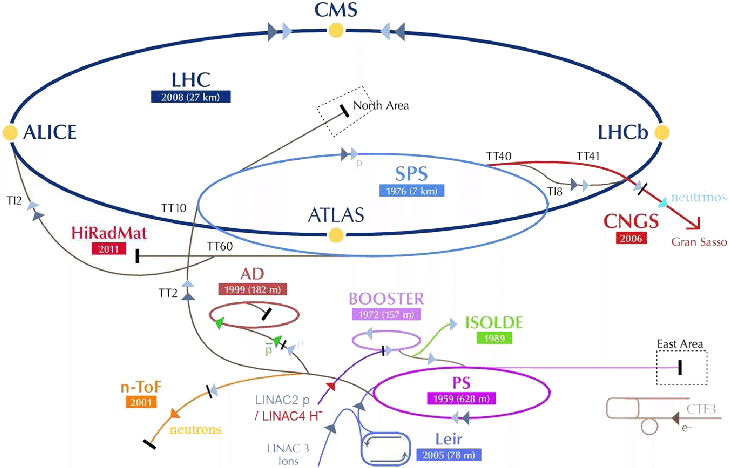
\includegraphics[width=0.8\textwidth]{schema-lhc.png}
			\caption[Schema LHC-a u CERN-u.]{\label{sl:schema-lhc}Schema LHC-a u CERN-u ~\cite{doktorat}. }
		\end{figure}
		Unutar samog ubrzivača, prije nego se sudare, putuju dvije visoko energizirane zrake čestica koje se gibaju brzinom bliskoj brzini svjetlosti~\cite{cern-lhc}. Zrake putuju unutar dvije odvojene cijevi u suprotnim smjerovima, a same cijevi su pod visokim vakuumom. Zrake su dovedene do brzine svjetlosti sa snažnim magnetskim poljem supravodljivih elektromagneta, koji su izgrađeni od zavojnica specijalnog materijala koji se ohladi na -271,3 \degree C, te omogućuje tok struje bez otpora. Iz tog razloga, cijeli akcelerator je umrežen u sustav tekućeg helija. Tisuće magneta raznih oblika i veličina usmjeravaju zrake kako bi točno prije sudara bile na istoj poziciji s većom vjerojatnošću sudara. Radi dobivanja osjećaja možemo reći da je taj sustav toliko precizan kao da ispalimo dvije igle na 10 km udaljenosti i želimo da se sudare.
		Sami sudari se događaju u 4 različita detektora ATLAS, CMS, ALICE i LHCb.
		
		\subsection{Kompaktni mionski solenoid}
		Kompaktni mionski solenoid (eng. Compact mion Solenoid, CMS) jedan je od 4 detektora koja postoje u LHC-u i ovo su njegove glavne karakteristike:
		\begin{itemize}
			\item kompaktnost – relativno je malen s obzirom na svoju masu
			\item mionski – napredni sustav za detekciju miona
			\item solenoid – supravodljivi solenoid
		\end{itemize}
	
		Kako je masa Higgsovog bozona slobodan parametar u SM-u, moralo je se tražiti u širokom energetskom rasponu od 100 GeV do 1 TeV. To je značilo da je detektor morao biti sposoban rekonstruirati i identificirati široki spektar objekata u finalnom stanju nakon raspada iz Higgsovog bozona. Također, detektor je morao biti dovoljno brz da analizira sve bitne događaje u sudarima, ali isto tako da preživi visoku radijaciju koja se događa u istim.
		Detektor se nalazi 100 m ispod malog francuskog sela Cessy. Dug 21 metar, 15 metara širok te 15 metara visok, CMS je kao veliki filter sa strukturom luka. Svaki sloj je zadužen za mjerenje nekih od svojstava različitih vrsta čestica. Detektor je izgrađen oko velikog magnetnog solenoida u obliku cilindra koji je ohlađen na -268,5 \degree C i generira polje od 4  T, što je oko 100 puta jače od magnetskog polja Zemaljske kugle.
		Čestice nastale u sudaru  (slika \ref{sl1:cms-scheme}) prvo prolaze kroz sustav tragova koji detektira putanju elektrona. Cijeli sustav tragova (eng. tracker) se nalazi pod jakim magnetskim poljem od 4 T kojim se može vrlo precizno zakriviti elektromagnetski nabijena čestica i izvući njena svojstva poput količine gibanja. Izvan sustav tragova nalazi se elektromagnetski kalorimetar (eng. Electromagnetic Calorimeter, ECAL) koji je namjenjen za detekciju i zaustavljanje fotona i elektrona. Idući sloj je hadronski kalorimetar (eng. Hadronic Calorimener, HCAL) zadužen za detekciju i zaustavljanje hadrona i nešto je slabijeg magnetskog polja od otprilike 3,8 T. Sve to obavijeno je supravodljivim solenoidom zaduženim za generiranje tako snažnih magnetskih polja. Konačno, 4 sloja mionskih detektora i željeznih barijera služe za detekciju i zaustavljanje miona pod magnetskim poljem od 2 T.
		\begin{figure}[H]
			\centering
			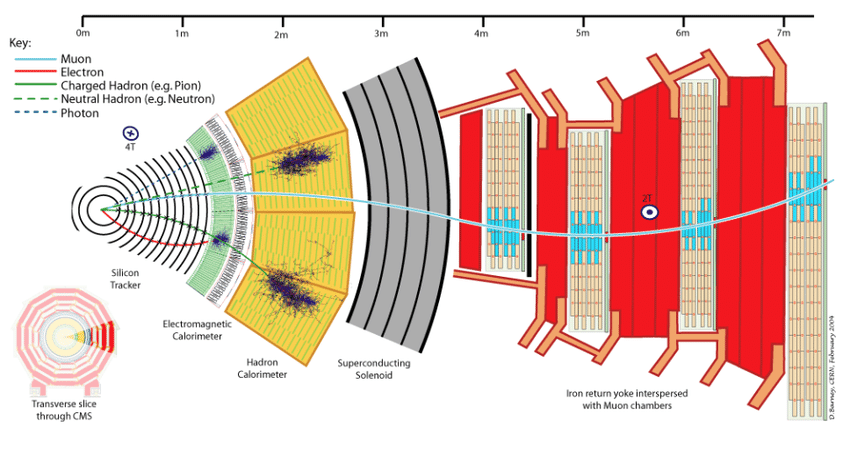
\includegraphics[width=0.8\textwidth]{cms-scheme.png}
			\caption[Saturn viđen u ultraljubičastom svjetlu.]{\label{sl1:cms-scheme}Schema presjeka kutnog isječka CMS detektora u CERN-u na kojemu su prikazani pojedini djelovi zaslužni za detektiranje i usporavanje određenih tipova elementarnih čestica~\cite{cern-slika}. }
		\end{figure}
	
		\subsubsection{Sistem okidača}
		Pri maksimalnom opterećenju u CMS-u sudari se događaju svakih 25 ns i nije moguće zabilježiti svaki od sudara~\cite{doktorat}. Zato je razvijen sustav okidača da bi zabilježili samo one događaje visokih energija  koji su nam posebno važni. Sustav je sastavljen od 3 koraka, gdje je L1 kompletno hardverski, dok su L2 i L3 softverski i objedinjeni su u visoko razinski okidač (eng. High level trigger, HLT). L1 razinski okidač spusti frekvenciju sudara koje prihvaćamo sa 40 MHz na samo 100 kHz. Kako ne bi miješao čestice iz dva različita sudara dozvoljen je odmak od samo 4 {$\mu$}s. Ako je uvjet zadovoljen šalje se na obradu u HLT sustav, a ako ne sudar se odbacuje. Zbog hardverske ograničenosti L1 sustav funkcionira samo na kalorimetrima i mionskim komorama
		Ako prođe L1 sustav okidača, sudar dolazi na softversku obradu koja zahtjeva ispunjavanje raznih uvjeta kao npr. postojanje dva izolirana elektrona.  U konačnici finalni ispis je samo 1 kHz frekvencije.
		
		\subsubsection{Rekonstrukcija čestica}
		Kao što smo već naveli, neke čestice imaju kratki vijek života i nemoguće ih je direktno detektirati. Iz tog razloga potrebno je napraviti rekonstrukciju čestica nastalih u procesu raspada naše željene čestice. Svaka čestica koja se detektira može nastati iz više elemenata i glavni cilj kod rekonstrukcije je povezati različite čestice u različitim detektorima s istom izvornom česticom. 
		Rekonstrukcija se može razbiti u 3 grube kategorije: praćenje tragova, algoritam klastera i algoritam čestičnog toka (eng. Particle-flow, PF).
		Praćenje tragova se odvija tako da se promatra trag čestice koja prolazi kroz magnetsko polje. Znajući snagu tog magnetskog polja možemo možemo izračunati komponente količine gibanja dane čestice. Sustav tragova može rekonstruirati putanje visoko-energiziranih miona, elektrona i hadrona. Također, od sustav tragova se očekuje da bude dovoljno precizan do na 10 $\mu$m, ali opet toliko nježan da ne utječe na samu česticu ~\cite{cern-sustav tragova}.
		Svrha algoritma klastera u kalorimetru je detektiranje te mjerenje energije i putanje stabilne neutralne čestice, odvajanje neutralnih čestica od nabijenih hadronskih čestica, te rekonstrukcija i identifikacija elektrona s popratnim zakočnim zračenjem fotona.
		PF algoritam objedinjuje cijelu rekonstrukciju u jednu cijelinu, no radi kompleksnosti ovog algoritma mi ćemo u ovom diplomskom opisati samo praćenje tragova miona i njihovu rekonstrukciju.
		
		S PF algoritmom možemo rekonstruirati 3 različita tipa mionskih kandidata:
		\begin{itemize}
			\item mioni koji stoje sami za sebe
			\item globalni mioni
			\item mioni tragova 
		\end{itemize}
		Nazivi su zapravo direktno povezani s dijelovima detektora u kojima su detektirani. Pa tako se mioni koji stoje sami dobivaju kao signali u mionskim komorama, mioni tragova kao signali u sustavu tragova, dok se globalni mioni dobivaju kao kombinacija ta dva signala. 
		Čak 99\% rekonstruiranih miona su globalni ili mioni tragova ~\cite{doktorat}. Globalni mioni popravljaju rezoluciju momenata, a mioni tragova popravljaju učinkovitost miona s niskom količinom gibanja koji ne uspiju u potpunosti prijeći cijeli CMS detektor. Globalni mioni i mioni tragova koji imaju isti trag se povezuju u jednog kandidata. mioni koji stoje sami za sebe inače imaju lošiju rezoluciju momenata i veću mješavinu kozmičkih miona nego globalni i mioni tragova.
		Naboj i količina gibanja PF miona se uzima iz prilagodbe funkcije tragova ako je količina gibanja manja od 200 GeV. Iznad te vrijednosti količina gibanja se uzima prema najmanjoj $\chi^{2}$ vjerojatnosti iz prilagodbe funkcije za različite tragove. Naravno da pri ovakvoj rekonstrukciju može doći do pogreške gdje se druge čestice rekonstruira kao mione i tada takvi procesi predstavljaju pozadinu.
		
		\newpage
		\section{Analiza kanala raspada \begin{math}
		\boldmath	{H \rightarrow ZZ^* \rightarrow 4\mu }\end{math} }
		Kako bi što bolje opisali svojstva Higgsovog bozona u SM-u jako je bitno da odredimo koje ćemo događaje promatrati proizvedene u CMS detektoru~\cite{doktorat}.
		Proces odabira događaja u ovoj analizi fokusira se na dobivanje što više signala Higgsovog bozona sa što manje pozadine. Također, veoma bitan korak ove analize je odabir varijabli kojima možemo odijeliti signal i pozadinu. Govoreći o pozadini postoje dvije vrste: reducibilna i ireducibilna pozadina. 
		Ireducibilna pozadina ima isto finalno stanje kao i signal, no nastala je iz drugog procesa SM-a. Npr. za naš kanal \begin{math}
		H \rightarrow ZZ^* \rightarrow 4\mu \end{math}, procesi ireducibilne pozadine bi bili \begin{math}
		gg \rightarrow ZZ
		\end{math} i \begin{math}
		q\bar{q}, \rightarrow ZZ
		\end{math}. Za razliku od ovakvih procesa koje nije teško simulirat, problem stvaraju procesi s reducibilnom pozadinom. To su procesi u kojem su finalni objekti krivo protumačeni u detektoru kao mioni nastali iz Z bozona. Zbog kompleksnosti simulacije takva pozadina se procjenjuje direktno iz podataka.
		
	
	
	
		\subsection{Podatci i Monte Carlo simulacije}
		Kao što smo već spomenuli u prošlom poglavlju, SM ne može predvidjeti masu Higgsovog bozona. Taj problem je znanstvenicima, prije otkrića Higgsovog bozona, zadavao velike glavobolje jer je cijela teorija SM-a počivala na činjenici da Higgsov bozon postoji i da ima nekakvu masu. Ipak, ustrajući u svojoj namjeri, da dokažu postojanje Higgsovog bozona, iz teorije začete još 50-ih godina prošlog stoljeća, znanstvenici su promatrali mase W bozona i top kvarka ~\cite{royal-sm}. Prema SM-u te čestice dolaze u mehanizmima proizvodnje Higgsovog bozona, a analizirajući mase tih  čestica suzilo se područje u kojima se traži Higgsov bozon .
		\begin{figure}[H]
			\centering
			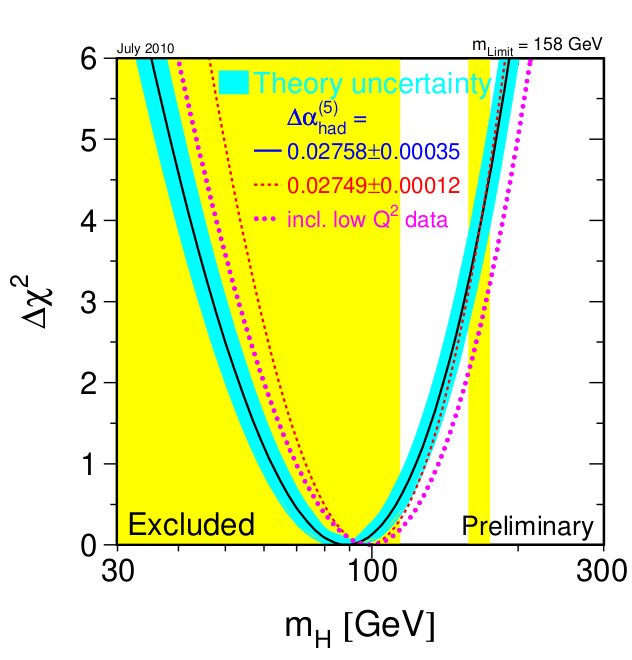
\includegraphics[width=0.8\textwidth]{sl2.png}
			\caption[Saturn viđen u ultraljubičastom svjetlu.]{\label{sl:sl2}Vjerojatnost postojanja Higgsovog bozona prikazan je kao funkcija \begin{math}
				\chi^2
				\end{math} u ovisnosti o masi Higgsovog bozona ~\cite{royal-sm}. }
		\end{figure}
		
	
		U radu iz 2003. godine ~\cite{royal-sm8} znanstvenici su eksperimentalnim mjerenjima odbacili hipotezu o postojanju mase Higgsovog bozona ispod 114 GeV, dok je 2011. odbačeno i postojanje mase Higgsovog bozona u intervalu od 158 do 173 GeV ~\cite{royal-sm9}. Uzimajući u obzir takva ograničenja konstruirala se likelihood funkcija najizglednije mase Higgsovog bozona, koju ćemo kasnije detaljnije opisati.  Kako predviđanje SM-a nije apsolutno, već ovisi i o drugim parametrima, na slici \ref{sl:sl2} su prikazane i parabole koje predstavljaju pogreške eksperimentalnih mjerenja tih parametara. Iako je najvjerojatnija vrijednost mase Higgsovog bozona u minimumu parabola, gore navedenim saznanjima, novo najizglednije područje pronalaska mase Higgsovog bozona postalo je interval od 114 do 158 GeV. Upravo takva saznanja su dovela znanstvenike da godinu dana kasnije dođu do najvažnijeg fizikalnog otkrića 21. stoljeća.
		
		\paragraph{Monte Carlo simulacije\newline}
		Idući vrlo bitan korak za oređivanje mase Higgsovog bozona i dokazivanju teorije SM-a, bile su izrade računalnih Monte Carlo simulacija. MC simulacije su računalni algoritmi koji se temelje na uzorkovanju slučajnih brojeva kako bi opisali nekakav problem koji može biti determinističke prirode (npr. rješavanje višedimenzionalnih integrala), ali i nedeterminističke (npr. kvantna mehanika)~\cite{mc-simulacije}. One su idealan način za simuliranje  stvarnih procesa koji se zbivaju u detektoru i gotovo jedini način za dokazivanje fizikalne teorije ovakve vrste. 
		Kao što su i realni procesi podijeljeni u nekoliko koraka, tako i MC simulacije moramo razdvojiti u različite etape.
		Prvi korak je simulacija proton-proton sudara. Teorija SM-a za p-p sudar nam daje vjerojatnosti nastanka pojedinih elementarnih čestica. U našem konkretnom slučaju, simulirao se sudar protonskih zraka energiziranih na 13 TeV. Kako neke elementarne čestice ne mogu egzistirati zasebno, poput gluona i kvarkova, idući potrebni korak je hadronizacija istih, te simuliranje jet-ova i čestičnog pljuska nastalog pri sudaru protonskih zraka. Kako protone ne šaljemo u kontinuiranom slijedu, već ih grupiramo u nakupine, pri prolasku jedne nakupine kraj druge može doći do tzv. preklapajućih nakupinskih međudjelovanja (eng. Pile up interactions)~\cite{pileup}. U tim procesima dolazi do zanimljivih, ali ne željenih procesa koji mogu omesti detektor. Zato je bitno simulirati i te događaje, kako ne bi došli do krivog zaključka o vjerojatnosti odvijanja procesa prema SM-u. 
		Nakon kreiranja događaja s odgovarajućim vjerojatnostima, potrebno je simulirati detektiranje istih. Trenutno najbolja platforma za simuliranje prolaska čestice kroz materiju je paket GEANT4~\cite{geant4}. Sofware razvijen 1998. godine, osim simuliranja detektora koji koristimo u čestičnoj fizici, koristi se u astrofizici pa čak i u medicini. 
		Posljednji korak MC simulacija je imitacija HLT-a i rekonstrukcija događaja s istim algoritmima koji se koriste i za prave podatke.
		Također, za razliku od stvarnih podataka gdje su signalni i pozadinski podatci izmiješani, s Monte Carlo simulacijama možemo vrlo elegantno odvojeno analizirati pozadine i signale.
		
		Zbog kompleksnosti izrada ovakvih MC simulacija, u ovom radu smo dobili već generirane podatke.
		
		\paragraph{Signalni Podatci\newline}
		Signalne procese koje smo razmatrali u ovom istraživanju su fuzija gluona (gg$\rightarrow$H), te fuzija vektorskih bozona. Zbog malog značaja na ukupni signal, ostale procese (WH, ZH, ttH, bbH) u proizvodnji Higgsovog bozona smo zanemarili.
		
		\paragraph{Pozadinski Podatci\newline}
		Kao što smo već objasnili na početku ovog poglavlja, ireducibilnu pozadinu nije teško simulirati jer SM predviđa vjerojatnosti nastanka takvih procesa. U naše istraživanje uključili smo kanal $q\bar{q}$$\rightarrow$ZZ$\rightarrow$4$\mu$ i kanal  gg$\rightarrow$ZZ$\rightarrow$4$\mu$.
		Simuliranje reducibilne pozadine je nešto kompliciraniji proces. Zbog kompleksnosti rekonstrukcije detektor može zabunom deklarirati neku drugu česticu kao mion~\cite{doktorat}. Ipak, vrlo efikasno, znanstvenici su kompleksnim tehnikama iz pravih podataka, ne utječući na konačan rezultat, uspjeli izvući vjerojatnost pojave ovakvih događaja. Sve procese ovakvog tipa ustaljeno je označavati sa Z+X. Valja naglasiti da se mi u ovom radu nismo koristili simuliranjem istih, već smo radili na dobivenim podatcima.
	
		\paragraph{Težina događaja\newline}
		Prije analize simuliranih podataka, bitan korak je dodjeljivanje težina svakom događaju. Težine događaja predstavljaju vjerojatnost odvijanja istog. Bez ovog koraka, svi događaji bi bili jednako vjerojatni i to bi uvelike narušilo stvarni prikaz podataka. Razlog tome leži u činjenici da mi kroz simulaciju generiramo puno više događaja, nego što je pravih izmjerenih podataka, jer želimo dobiti dovoljno dobro populiran fazni prostor za predviđanje različitih svojstava Higgsovog bozona.
		Težine događaja se računaju prema formuli:	
		\begin{equation}\label{eqn:tezina}
		w_{događaja} =  \frac{L_{int}*\sigma*BR*{SF}}{\sum_{svi događaji} w_{generator}}
		\end{equation}
		U jednadžbi \ref{eqn:tezina} ${L_{int}}$ predstavlja integrirani luminozitet, a $\sigma$ udarni presjek. Integrirani luminozitet je veličina obrnuto proporcionalna udarnom presjeku i govori nam koliko je ukupno podataka prikupljeno. Što je veći luminozitet, veća je šansa da će doći do sudara čestica. U ovom radu, podatci su prikupljeni u periodu 2016.-2018. godine i ukupan integrirani luminozitet je bio 137~$\mathrm{fb}^{-1}$ slika \ref{sl:luminozitet}.  BR predstavlja omjer grananja koji nam govori o vjerojatnosti raspada čestica na lakše čestice, a SF je faktor skaliranja koji moramo uvesti kako bi opisali sve ostale faktore koji utječu na konačne podatke. Konačno sve je normalizirano na ukupnu težinu s izrazom u nazivniku. 
		
		\subsection{Statistička analiza}
		\subsubsection{Funkcija gustoće vjerojatnosti}
		Idući korak nakon simulacije događaja u detektoru je pronaći model, tj. funkciju koja najbolje opisuje naše simulirane podatke. Takve vrste funkcija se zovu funkcije gustoće vjerojatnosti (eng. Probability density function, PDF). PDF je funkcija koeficijenta prve derivacije raspodjelne funkcije F(x) u točkama gdje je x definiran \begin{math}
		f(x)=\frac{\partial F(x)}{dx}
		\end{math}. Za kontinuiranu vrijednost od x, površina ispod grafa PDF-a u intervalu od $x_L$ do $x_U$ predstavlja vjerojatnost da neki slučajno generiran broj prema danom modelu F(x) upadne u dani interval~\cite{pdf}.
		\begin{figure}[H]
			\centering
			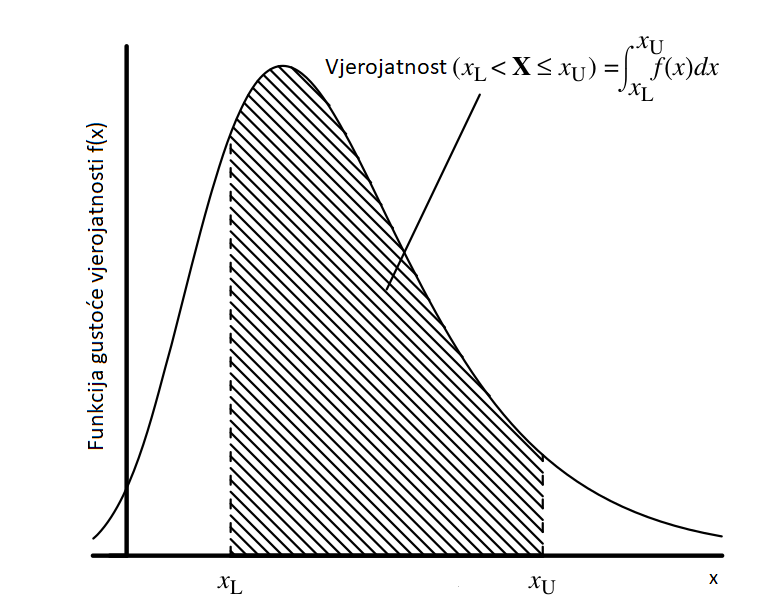
\includegraphics[width=1.0\textwidth]{sl4.png}
			\caption[Saturn viđen u ultraljubičastom svjetlu.]{\label{sl:pdf}PDF funkcija. Slika preuzeta iz ~\cite{pdf}}
		\end{figure}
	
		\subsubsection{Likelihood}
		Kada odaberemo pravi PDF za opisivanje simuliranih podataka, njene parametre treba namjestiti tako da funkcija prati podatke. Taj postupak se zove prilagodba funkcije na podatke(eng. fit). Ako pretpostavimo da su svi događaji međusobno nezavisni, onda je vjerojatnost za N događaja dana kao produkt vjerojatnosti svakih od pojedinačnih događaja:
		\begin{equation}
		P(x;\theta) = P(x_1 ; \theta) P(x_2 ; \theta) \cdot \cdot \cdot P(x_N ; \theta) = \prod P(x_i ; \theta)
		\end{equation}
		Kada se varijabla x zamjeni varijablom \begin{math}
		x^{OBS}
		\end{math} tada P nije više PDF, već likelihood funkcija  koja se označava sa \begin{math}
		L (x^{OBS}; \theta)
		\end{math}. Vjerojatnost odvijanja N nezavisnih događaja je dana s:
		\begin{equation}
		L(x; \theta) = \prod f(x_i; \theta)
		\end{equation}
		Maximum likelihood estimator \begin{math}
		\hat{\theta}
		\end{math} je vrijednost $\theta$ za koji je funkcija likelihooda postiže najveću vrijednost, tj. za koju je funkcija najvjerojatnija. Traženje maksimuma se može provesti na standardan način,deriviranjem funkcje L i izjednačavanjem s 0, no ipak je bolje tražiti maksimum log-likelihood funkcije:
		\begin{equation}
		ln L(x; \theta) = \sum ln f(x_i; \theta)
		\end{equation}
		jer je operacija množenja zamijenjena operacijom zbrajanja koja je računalno puno jednostavnija.
		Ovdje valja naglasiti da procjena maksimumlikelihooda nije najvjerojatnija vrijednost traženog parametra, već je najbolja procjena naših uzorkovanih podataka.
		
		\begin{figure}[H]
			\centering
			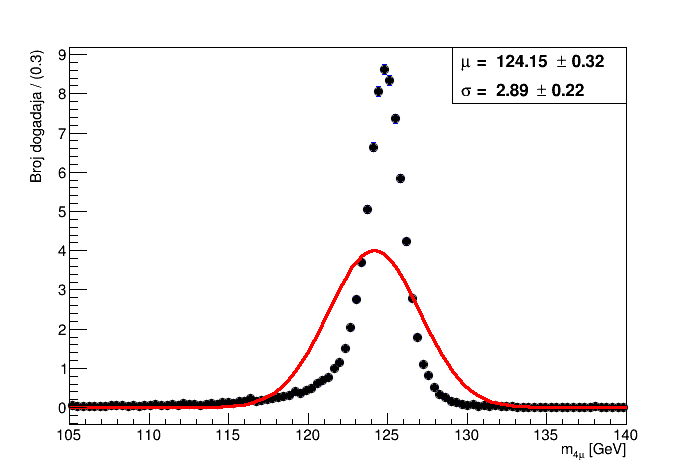
\includegraphics[width=1.0\textwidth]{gauss-fit-23-7-final-weighted.png}
			\caption[Saturn viđen u ultraljubičastom svjetlu.]{\label{sl:gauss-fit} Prilagodba podataka na Gaussovu krivulju}
		\end{figure}
		Prvo smo pokušali prilagoditi simulirane podatke na Gaussovu krivulju (slika \ref{sl:gauss-fit}). Uzimajući srednju vrijednost koja varira u intervalu [105,140], te standardnu devijaciju $\sigma$ [0.1, 5.0] uočavamo loše slaganje sa simuliranim podatcima, posebno oko 125 GeV. Ipak Gussian je dobar temelj za nastavak rada, jer vidimo simetričnu raspodjelu podataka oko 125 GeV.
		
		Važno je istaknuti da simulirani podatci prema SM-a nisu podjeljeni u manje sekcije (eng. binned data) već ih promatramo kao kontinuirani spektar vrijednosti. Ipak radi grafičkog prikaza, koji nam uvelike olakšava percipiranje raspodjele podataka, moramo ih grupirati u manje skupine kako bi se graf mogao konstruirati. U našem konkretnom slučaju na slici \ref{sl:gauss-fit} podatci su podjeljenu u koševe (eng. bin)  veličine (širine) 0.3 GeV. Ovakav pristup izrade grafova je korišten u cijelom diplomskom radu s različitim širinama koševa.
		
		\begin{figure}[H]
			\centering
			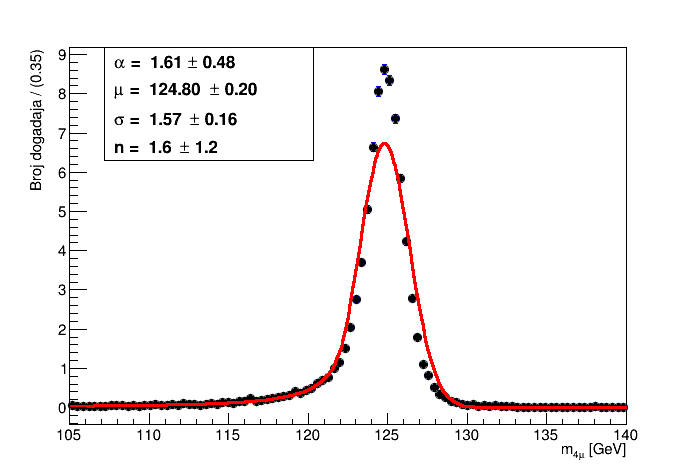
\includegraphics[width=1.0\textwidth]{CBFit-23-7-final-weight.png}
			\caption[Saturn viđen u ultraljubičastom svjetlu.]{\label{sl:cbfit} Prilagodba podataka na Crystall ball krivulju}
		\end{figure}
		Idući pokušaj je bio s Crystal ball funkcijom koja se inače koristi u opisivanju raznih procesa u fizici visokih energija. Sama funkcija u svojoj jezgri sadrži Gaussian, a drugi dio je recipročna potencijalna funkcija n-te potencije koja se pojavljuje ispod određenih vrijednosti $\alpha$. Svi parametri su varirani i pušteni da dostižu svoje granične vrijednosti, no ipak zadovoljavajuće slaganje s izmjerenim podatcima nije postignuto.
		
		Konačno, funkcija koja je najbolje opisala signalne simulirane podatke bila je double Crystal ball:
		\begin{align}
		\begin{split}
		dCB(x; \alpha_1, \alpha_2, n_1, n_2, \mu, \sigma)={}& N \cdot \begin{cases}
		exp(- \frac{(x-\mu)^2}{2\sigma^2}),& -\alpha_1 <\frac{x-\mu}{\sigma}< \alpha_2\\
		A \cdot (B- \frac{x-\mu}{\sigma})^{-n_1},& \frac{x-\mu}{\sigma} < - \alpha_1\\
		E \cdot (F + \frac{x-\mu}{\sigma})^{-n_2},& \frac{x-\mu}{\sigma} >  \alpha_2
		\end{cases}\\
		&A = (\frac{n_1}{|\alpha_1|})^{n_1} \cdot exp(- \frac{|\alpha_1|^2}{2}), \\
		&B = \frac{n_1}{|\alpha_1|} - |\alpha_1|, \\
		&C = \frac{n_1}{|\alpha_1|} \cdot \frac{1}{n_1 - 1} \cdot exp(- \frac{|\alpha_1|^2}{2}), \\
		&D = \sqrt{\frac{\pi}{2}} (1+erf(\frac{|\alpha_1|}{\sqrt{2}})) \\
		&N = \frac{1}{\sigma (C+D)}, \\
		&E = (\frac{n_2}{|\alpha_2|})^{n_2} \cdot exp(- \frac{|\alpha_2|^2}{2}), \\
		&F = \frac{n_2}{|\alpha_2|} - |\alpha_2|
		\end{split}
		\end{align}
		
		
		Istom funkcijom koristili su se znanstvenici u CERN-u prilikom otkrivanja mase Higgsovog bozona. To je bila najjednostavnija, a ujedno i najrobusnija funkcija koja je mogla dovoljno dobro opisati simulirane podatke~\cite{atlas-rad}. Sačinjena je od jezgre Gaussiana srednje vrijednosti(eng. mean) $\mu$ i širine $\sigma$, te recipročnih potencijalnih funkcija n-tih stupnjeva, $n_{1}$ za vrijednosti niže od -$\alpha_{1}$ te $n_{2}$ za vrijednosti više od $\alpha_{2}$. Parametri pragova (eng. Threshold)  $\alpha_{1,2}$ određuju u kojoj točki Gauss prelazi u polinomnu funkciju.
		\begin{figure}[H]
			\centering
			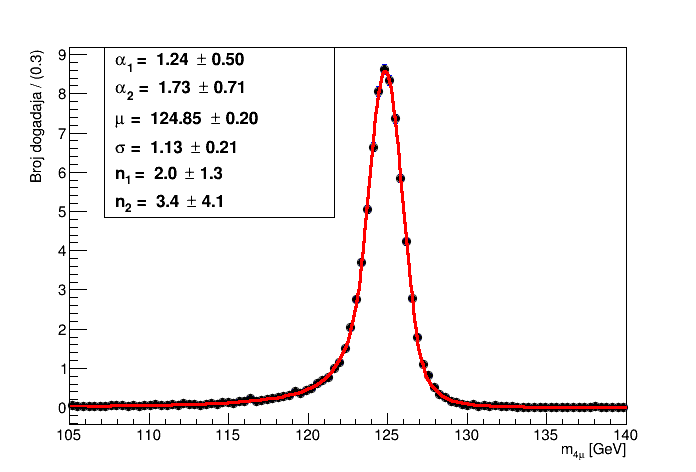
\includegraphics[width=1.0\textwidth]{dCB-23-7-final-weighted.png}
			\caption[Prilagodba simuliranih podataka fuzije gluona na dCB funkciju definiranu u tekstu.]{\label{sl:dcbfit} Prilagodba simuliranih podataka fuzije gluona na dCB funkciju definiranu u tekstu.}
		\end{figure}
	
		Ovim prilagođavnjem simularnih podataka smo pokazali da double Crystal ball funkcija najbolje opisuje raspodjelu mase Higgsovog bozona oko srednje vrijednosti od 125 GeV prema predviđanju teorije SM-a.
	
		Na isti način, dCB funkciju smo prilagodili i na signal u kanala vektor bozon fuzije slika \ref{sl:dcbfit-vbfh}:		
		\begin{figure}[H]
			\centering
			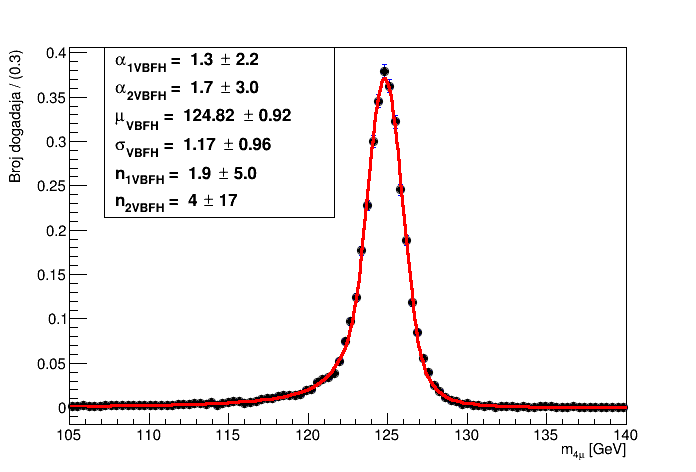
\includegraphics[width=1.0\textwidth]{signal-vbfh-weighted1.png}
			\caption[Prilagodba simuliranih podataka fuzije vektorskih bozona na dCB funkciju definiranu u tekstu.]{\label{sl:dcbfit-vbfh} Prilagodba simuliranih podataka fuzije vektorskih bozona na dCB funkciju definiranu u tekstu.}
		\end{figure}
		Kako je slična funkcija opisala i vektor bozon fuziju, zbog malog ukupnog doprinosa mi smo taj signal sumirali kanalu gluon fuzije. Pritom smo u obzir uzeli i normalizaciju te funkcije.
	
		Cijeli postupak prilagodbe podataka na double Crystal ball funkciju ponovljen je i za simulirane podatke u kojima se masa pretpostavlja na vrijednosti 120, 124, 126 i 130 GeV. Uzimajući dobivene srednje vrijednosti s obzirom na različite mase, uočena je linearna ovisnost parametra $\mu$ o m$_{\mathrm{H}}$ (slika \ref{sl:sl5}).
		
		 
		\begin{figure}[H]
			\centering
			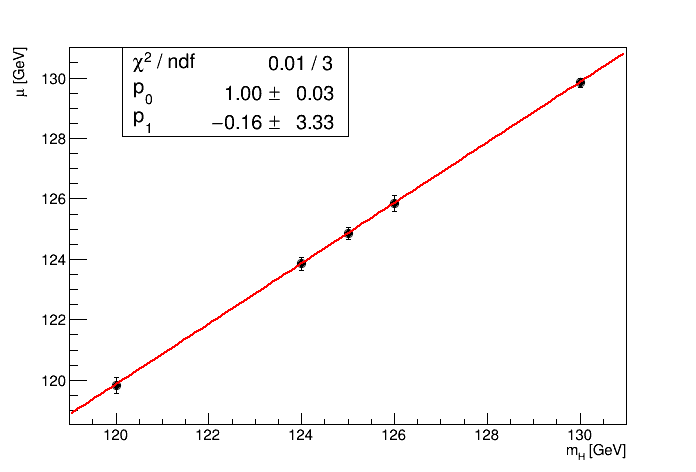
\includegraphics[width=1.0\textwidth]{fit-mH-19-8.png}
			\caption[Fit linearne funkcije na srednje vrijednosti za različite mase Higgsovog bozona.]{\label{sl:sl5} Fit linearne funkcije na srednje vrijednosti za različite mase Higgsovog bozona.}
		\end{figure}
	
		Tako smo zapravo parametrizirali masu Higgsovog bozona kao linearnu funkciju srednjih vrijednosti funkcija prilagođenih za različite simulirane podatke. 
		Isti postupak parametrizacije smo napravili i za ostale parametre double crystal ball funkcije. Uočeno je konstantno ponašanje svakog parametra u ovisnosti o masi Higgsovog bozona, što nam je uvelike olakšalo i smanjilo vrijeme trajanje prilagodbe funkcije na podatke.
		
		\begin{figure}[H]
			\centering
			\begin{subfigure}[b]{0.7\textwidth}
				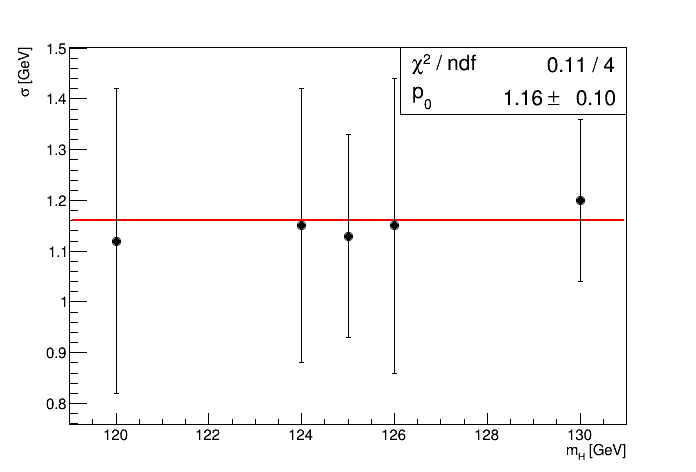
\includegraphics[width=\textwidth]{fitanje-sigma-1-8.png}
				\caption{}
				\label{fig:sigma}
			\end{subfigure}
		
			~ %add desired spacing between images, e. g. ~, \quad, \qquad, \hfill etc. 
			%(or a blank line to force the subfigure onto a new line)
			\begin{subfigure}[b]{0.49\textwidth}
				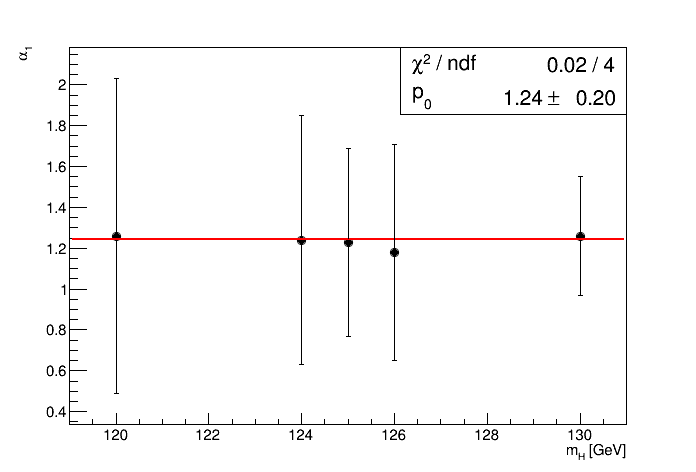
\includegraphics[width=\textwidth]{fitanje-alpha1-1-8.png}
				\caption{}
				\label{fig:alpha}
			\end{subfigure}
			\begin{subfigure}[b]{0.49\textwidth}
				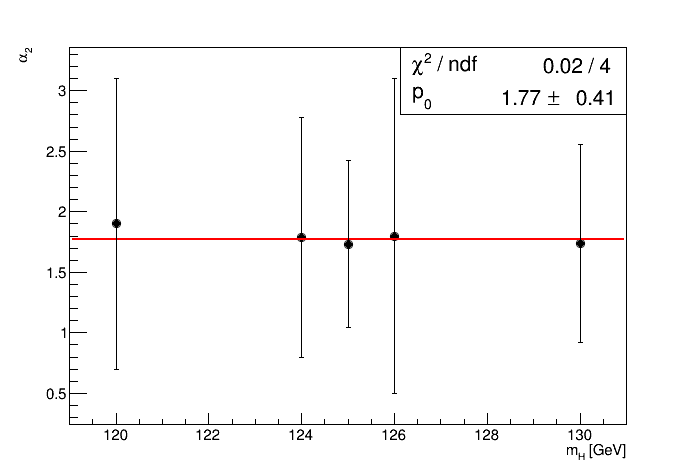
\includegraphics[width=\textwidth]{fitanje-alpha2-4-8.png}
				\caption{}
				\label{fig:alpha2}
			\end{subfigure}
		
			\begin{subfigure}[b]{0.49\textwidth}
				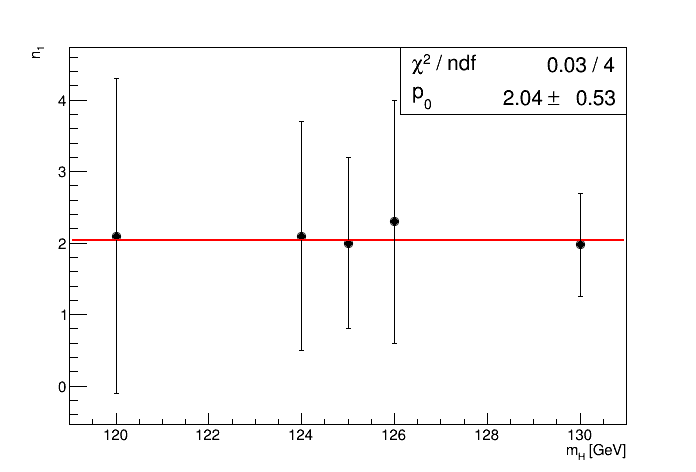
\includegraphics[width=\textwidth]{fitanje-n1-4-8.png}
				\caption{}
				\label{fig:n}
			\end{subfigure}
			\begin{subfigure}[b]{0.49\textwidth}
				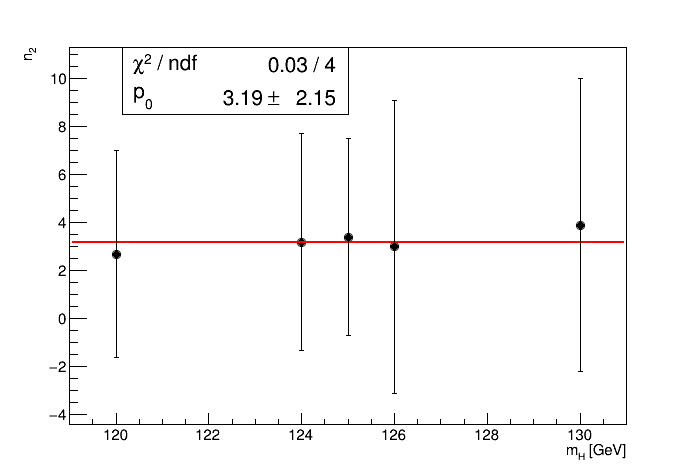
\includegraphics[width=\textwidth]{fitanje-n2-4-8.png}
				\caption{}
				\label{fig:n2}
			\end{subfigure}
			~ %add desired spacing between images, e. g. ~, \quad, \qquad, \hfill etc. 
			%(or a blank line to force the subfigure onto a new line)
			\caption{ a)Prilagođanje konstantne funkcije standardne devijacije $\sigma$ za različite vrijednosti mase Higgsovog bozona.	b)Prilagođanje konstantne funkcije parametra $\alpha_{1}$ za različite vrijednosti mase Higgsovog bozona.		c)Prilagođanje konstantne funkcije parametra $\alpha_{2}$ za različite vrijednosti mase Higgsovog bozona.		d)Prilagođanje konstantne funkcije parametra n$_{\mathrm{1}}$ za različite vrijednosti mase Higgsovog bozona.		e)Prilagođanje konstantne funkcije parametra n$_{\mathrm{2}}$ za različite vrijednosti mase Higgsovog bozona.}\label{fig:grafovi-1}
		\end{figure}
		
		
		Takav ishod je značio da u konačnom prilagođavanju na podatke ti parametri ne ovise o traženoj masi Higgsovog bozona m$_{\mathrm{H}}$.
		
		Za razliku od signala, koji je zahtijevao dosta kompliciranu funkciju za najbolji opis simuliranih događaja, pozadine su opisane nešto jednostavnijim funkcijama.
		Pozadina koja predviđa kanal raspada gg$\rightarrow$ZZ$\rightarrow$4$\mu$ opisana je linearnom funkcijom (polinomom prvog reda),  a ona koja previđa kanal raspada $q\bar{q}$$\rightarrow$ZZ$\rightarrow$4$\mu$ opisana je kvadratnom funkcijom (polinomom drugog reda) slika \ref{fig:grafovi-2}. Landau funkciju smo odabrali za onu koja opisuje ireducibilnu pozadinu Z+X, no kao što smo već naglasili, nju nismo simulirali već smo radili s dobivenim podatcima.
		
				\begin{figure}[H]
			\centering
			\begin{subfigure}[b]{0.9\textwidth}
				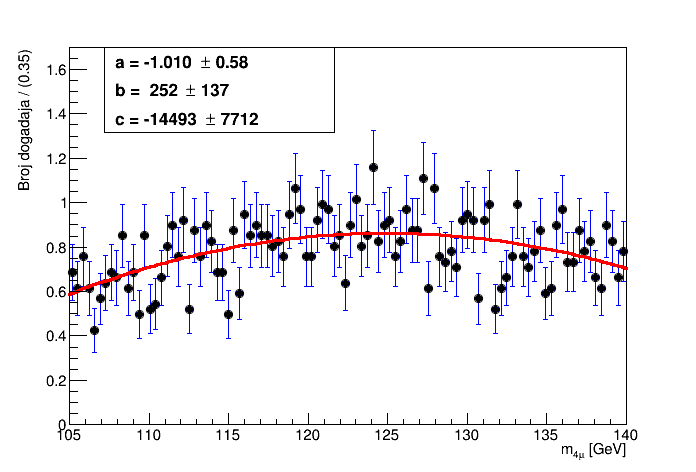
\includegraphics[width=\textwidth]{background-qqZZ-weighted.png}
				\caption{}
				\label{fig:bckg-zz}
			\end{subfigure}
			~ %add desired spacing between images, e. g. ~, \quad, \qquad, \hfill etc. 
			%(or a blank line to force the subfigure onto a new line)
			\begin{subfigure}[b]{0.9\textwidth}
				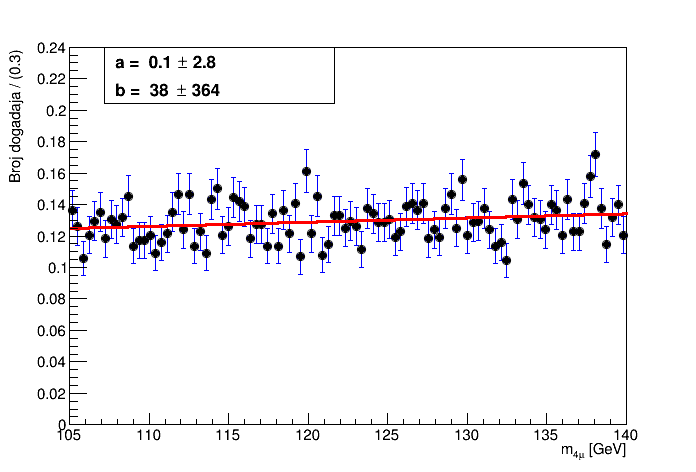
\includegraphics[width=\textwidth]{background-ggto4mu-weighted.png}
				\caption{}
				\label{fig:bckg-gg}
			\end{subfigure}
			~ %add desired spacing between images, e. g. ~, \quad, \qquad, \hfill etc. 
			%(or a blank line to force the subfigure onto a new line)
			\caption{a) Kvadratna funkcija prilagođena na simulirane podatke pozadine $q\bar{q}$$\rightarrow$ZZ$\rightarrow$4l.	b)Linearna funkcija prilagođena na simulirane podatke pozadine gg$\rightarrow$ZZ$\rightarrow$4l.}\label{fig:grafovi-2}
		\end{figure}
		
		Iz grafova su jasno vidljive velike oscilacije podataka, što znači i kada bi odabrali nekakvu kompleksnu funkciju za opisivanje simuliranih pozadinskih događaja, takva funkcija bi vjerojatno bila loša za neke drugačije generirane podatke istog modela.
		Unatoč velikim oscilacijama, ovakva procjena funkcija za opisivanje pozadine je dovoljno dobra jer prije samog otkrića Higgsovog bozona dok se čestica još tražila u drugim energetskim područjima, pozadina nije imala značajnije oscilacije koje bi ukazivale da se ponaša drugačije oko 125 GeV ~\cite{royal-sm8, royal-sm9}. Iako ova odluka sa sobom donosi određenu sistematsku pogrešku, radi kompleknosti problema, ista u ovom diplomksom radu neće biti detaljno obrađena već će se uzeti u obzir s jednostavnim računom što će rezultirati u dosta konzervativnijem rezultatu.  
		
		
		Uz same parametre funkcija koje opisuje signale i pozadine, bitan parametar koji izvlačimo iz simuliranih podataka je i integral funkcije. Taj podatak nam govori koliko se relativnih događaja svakog procesa odvije s obzirom na sve promatrane procese u detektoru. Njega možemo izračunati direktnim integriranjem funkcije nakon prilagodbe funkcije na simulirane podatke ili pak sumiranjem svih težina događaja tog procesa.
		U tablici \ref{tab:integrali} prikazani su integrali funkcije s obzirom na proces.
		\begin{table}[H]
			\centering
			\caption[Integrali prilagođenih funkcija s obzirom na dani proces]{\label{tab:integrali}Integrali prilagođenih funkcija s obzirom na dani proces}
			\begin{tabular}{?l|l|l?}
				\hlineRub
				tip                       & proces                               & Integral (\%)      \\ \hline
				\multirow{2}{*}{Signal}   & ggH                              & 77.56 			(36.4\%) \\
				& VBFH                              & 6.72(3.2\%)     \\ \hline
				\multirow{3}{*}{Pozadina} & $q\bar{q}$ $\rightarrow$ZZ$\rightarrow$4l & 82.25(38.6\%)     \\
				& gg$\rightarrow$ZZ$\rightarrow$4l                             & 9.24(4.3\%)     \\
				& Z+X(landau)                          & 37.3(17.5\%)     \\ 
				\hlineRub
			\end{tabular}
		\end{table}
		Za razliku od tima znanstvenika u CERN-u koji analizairaju gotovi svaki proces koji predviđa SM, mi u ovom istraživanju radimo s 2 najvažnija signalna i 3 pozadinska procesa. Iz tog razloga, integral ukupnog modela možemo promatrati kao sumu pojedinačnih integrala. Postotci u tablici \ref{tab:integrali} nam govore o udjelu pojedinog procesa u ukupnom modelu. Taj postotak smo promatrali kao udio pojedinog integrala tj. težine procesa s obzirom na sumu svih integrala, tj. težina procesa.
		Radi gotovo identičnog PDF-a, proces vektor bozon fuzije smo pribrojili kanalu proizvodnje fuzije gluona. Ostali signalni procesi su jako malog utjecaja, pa nisu bili dio ovog istraživanja.
		Promatrajući za mase 120, 124, 125, 126 i 130 GeV uočena je linearna ovisnost signalnog integrala prikazanog na slici \ref{sl:sl6}. Time smo parametrizirali još jednu varijablu kao linearnu funkciju mase Higgsovog bozona.
		
		\begin{figure}[H]
			\centering
			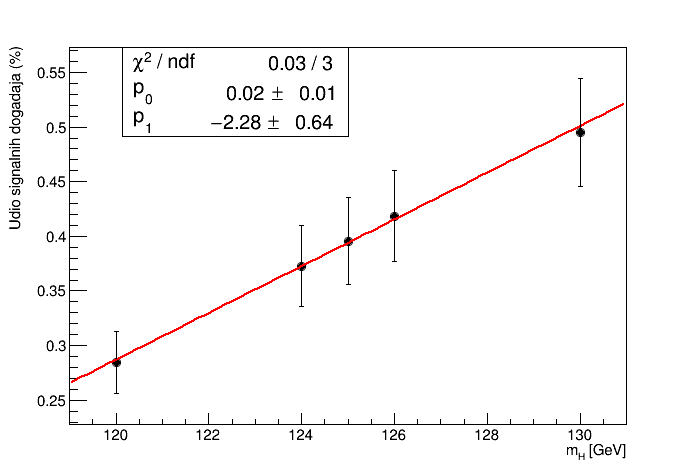
\includegraphics[width=0.9\textwidth]{fit-integrali-19-8.png}
			\caption[Fit linearne funkcije na integrale funkcija za različite mase Higgsovog bozona.]{\label{sl:sl6} Fit linearne funkcije na integrale funkcija za različite mase Higgsovog bozona.}
		\end{figure}
		
		
		\subsection{ROOT i RooFit}
		Simulirani podatci pozadina i signala su izgenerirani u konačan oblik ".root" datoteke. Ekstenzija takve datoteke dolazi od ROOT , objektno orijentiranog programa te biblioteke razvijene u CERNU-u. Primarna namjena joj je bila za analizu podataka u čestičnoj fizici, no danas se također, koristi u astronomiji i rudarenju podataka~\cite{roofit}. Glavna stavka ROOT datoteka je ta, da za pohranu podataka koristi stablo(tzv. Tree) koje ima svoje podkategorije grane(eng. Branches) i listove(eng. Leaves).  Stablo je vrlo elegantan način za spremanje podataka jer izbjegava probleme alociranja memorije kod stvaranja objekata, a samo spremanje se obavlja vrlo brzo. 
		Uz ROOT biblioteku koristili smo se ponajviše njenom ekstenzijom RooFit s kojom se na vrlo elegantan način rješavaju kompleksni problemi prilagodbe podataka na nekakav model. ROOT biblioteku smo implementirali s C++ koji je i dan danas jedan od najbržih računalnih programa na svijetu.
		
		\subsection{Ukupni model}
		Nakon određivanja funkcija koje se najbolje prilagođavaju na signalne i pozadinske podatke, napravili smo ukupan model koristeći se RooAddPdf metodom iz RooFit biblioteke ~\cite{rooaddpdf}. 
		Ukupni signalni model, označen crvenom bojom, možemo definirati kao:
		\begin{equation}\label{eq:signal}
		PDF_{SIG}=N_{ggH} \cdot dCB(x;\alpha_{1}, \alpha_{2}, n_{1}, n_{2}, \mu, \sigma) + N_{VBFH} \cdot dCB(x;\alpha_{1}, \alpha_{2}, n_{1}, n_{2}, \mu, \sigma)
		\end{equation}
		, no kako dCB ima gotovo identične parametre za oba signala, jednadžbu \ref{eq:signal} možemo zapisati kao:
		\begin{equation}
		PDF_{SIG}=(N_{ggH} + N_{VBFH}) \cdot dCB(x;\alpha_{1}, \alpha_{2}, n_{1}, n_{2}, \mu, \sigma)
		\end{equation}
		Pozadina $q\bar{q}$$\rightarrow$ZZ$\rightarrow$4l označena je zelenom, gg$\rightarrow$ZZ$\rightarrow$4l narančastom, a Z+X žutom bojom. Ukupni model pozadine smo označili crnom bojom i dan je formulom:
		\begin{equation}
		PDF_{BKG}=N_{qqZZ} \cdot P_1 (a_{1},b_{1},c_{1}) + N_{ggZZ} \cdot P_2 (a_{2},b_{2}) + N_{Z+X} \cdot Landau(\mu, \sigma)
		\end{equation}
		Ukupni model možemo zapisati kao sumu signalnog i pozadinskog PDF-a:
		\begin{equation}
		PDF=\mu * PDF_{SIG} + PDF_{BKG}
		\end{equation}
		,gdje $\mu$ predstavlja jačinu signala koja je definirana kao omjer stvarnog udarnog presjeka i udarnog presjeka koji predviđa SM \begin{math}
		\mu = \frac{\sigma}{\sigma_{SM}}
	\end{math} ~\cite{doktorat}.
		
		Umjesto učitavanja dosadašnjih podataka, za testiranje modela sami smo generirali nove podatke prema ukupnom modelu. Cilj je bio pokazati da bez obzira na odabranu srednju vrijednost mase, ukupni model će imati isti oblik i iste odnose značajnih parametara.
						\begin{figure}[H]
			\centering
			\begin{subfigure}[H]{0.7\textwidth}
				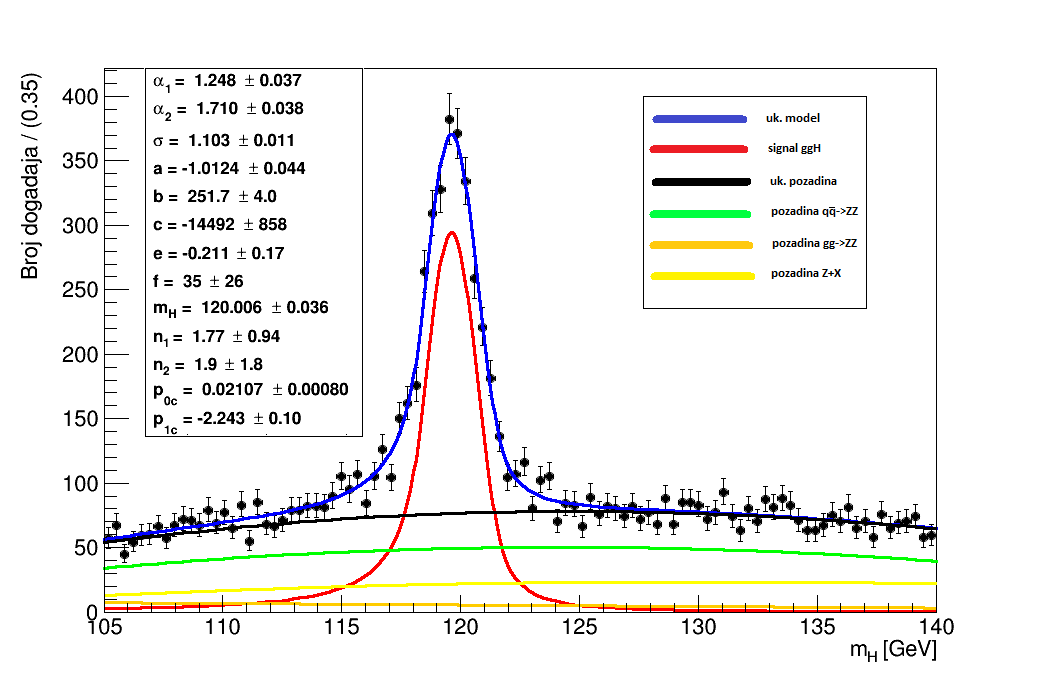
\includegraphics[width=\textwidth]{simulation-120.png}
				\caption{}
				\label{fig:model-120}
			\end{subfigure}
			~ %add desired spacing between images, e. g. ~, \quad, \qquad, \hfill etc. 
			%(or a blank line to force the subfigure onto a new line)
			\begin{subfigure}[b]{0.7\textwidth}
				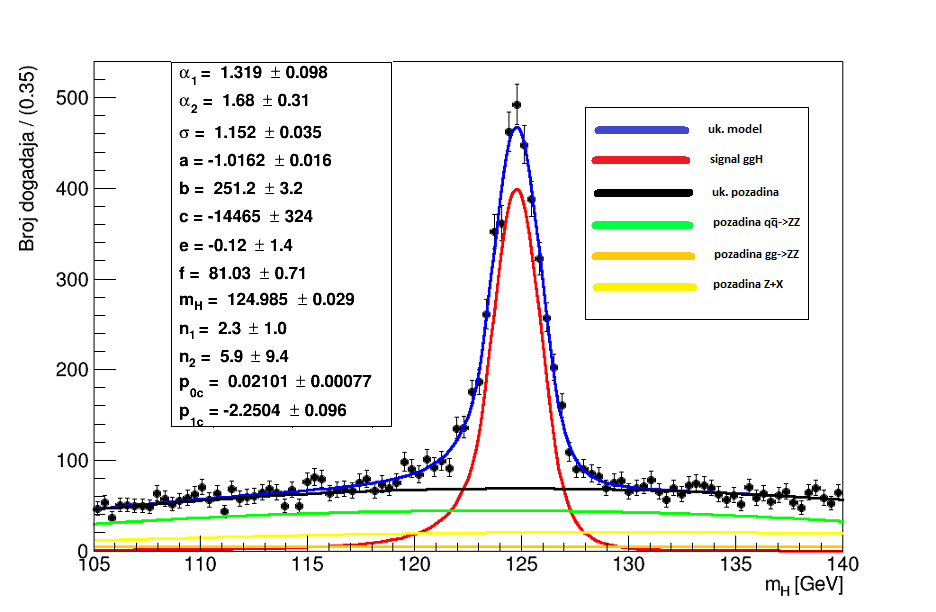
\includegraphics[width=\textwidth]{simulation-125.png}
				\caption{}
				\label{fig:model-125}
			\end{subfigure}
			\begin{subfigure}[b]{0.7\textwidth}
				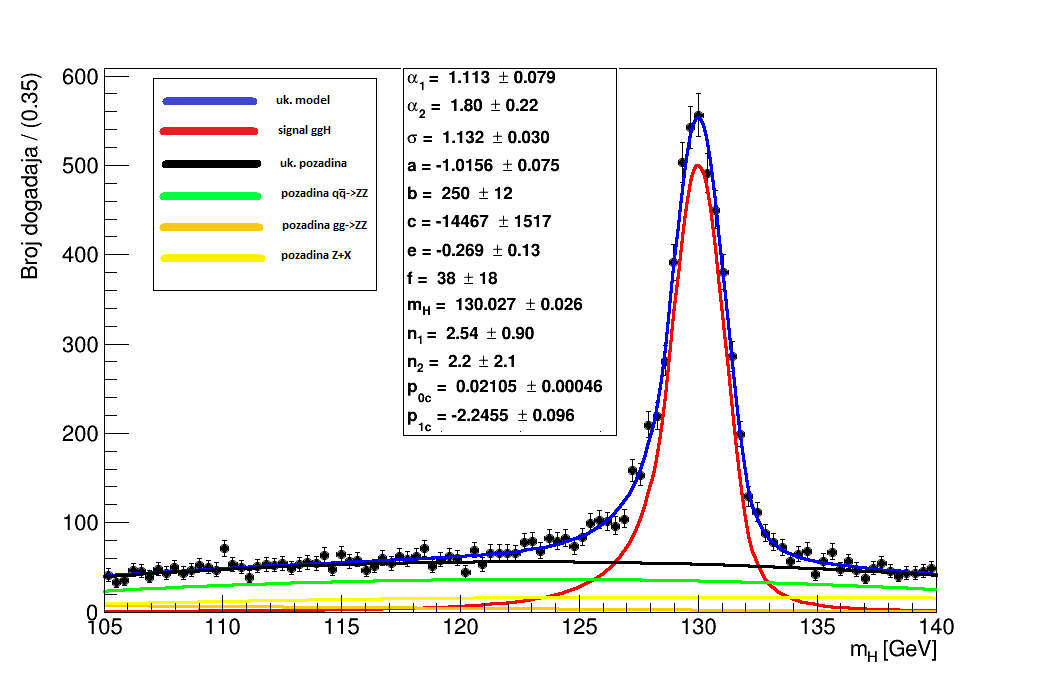
\includegraphics[width=\textwidth]{simulation-130.png}
				\caption{}
				\label{fig:model-130}
			\end{subfigure}
			~ %add desired spacing between images, e. g. ~, \quad, \qquad, \hfill etc. 
			%(or a blank line to force the subfigure onto a new line)
			\caption{a) Model prilagođen za masu Higgs-a 120 GeV.	b)Model prilagođen za masu Higgs-a 125 GeV.	c)Model prilagođen za masu Higgs-a 130 GeV.}\label{fig:grafovi-3}
		\end{figure}		
		
		
		\newpage
		\section{Rezultati}
		Posljednji korak u dokazivanju teorije SM-a i mjerenju mase Higgsovog bozona je prilagodba naše funkcije na stvarne podatke dobivene u periodu 2016. do 2018. godine. Svi parametri našeg modela, osim srednje vrijednosti i jačine signala, su fiksirani. SM model ne predviđa masu Higgsovog bozona i zato bi se naša funkcija trebala prilagoditi sa srednjom vrijednošću kolika god ona bila jer je parametrizirana preko same mase Higgsovog bozona. Isto tako ostavljamo mogućnost da je predviđanje broja događaja SM-a pogrešno pa ćemo prilagođavanjem i jačine signala provjeriti tu hipotezu.
		
		\begin{figure}[H]
			\centering
			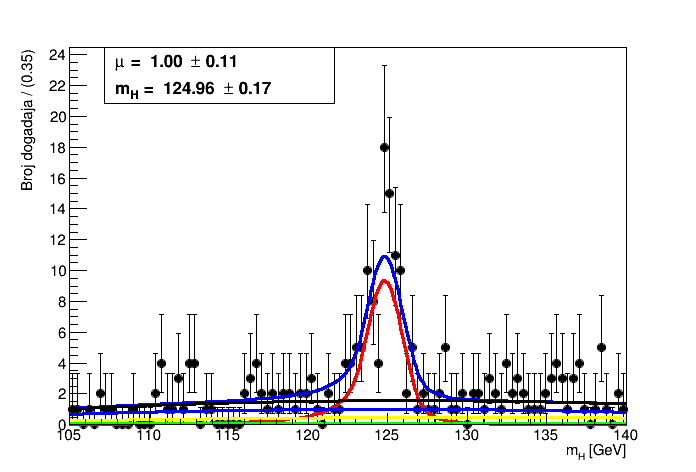
\includegraphics[width=0.9\textwidth]{27-8.png}
			\caption[Saturn viđen u ultraljubičastom svjetlu.]{\label{sl:sl7} Prilagodba konstruiranog modela na stvarne podatke}
		\end{figure}
		 
		 Vrijednost jačine signala je 1.00$\pm$0.11, što znači da se naš model slaže s teorijskim predviđanjem do na pogrešku mjerenja. Ovdje se moramo prisjetiti da smo zanemarili neke rijeđe procese nastajanja Higgsovog bozona, ali s obzirom na veliku grešku mjerenja njihovim uključivanjem u model zaključak se nebi značajno promjenio.
		 
		 Kao što smo već objasnili, svi dosadašnji grafovi su bili samo lijepi prikaz podataka, gdje smo promatrali koliko ima podataka u nekom rasponu koševa. No interesantno je prikazati i minimiziranje loglikelihood funkcije, gdje podaci nisu prisilno raspoređivani u određene koševe energija.
		 
		 \begin{figure}[H]
		 	\centering
		 	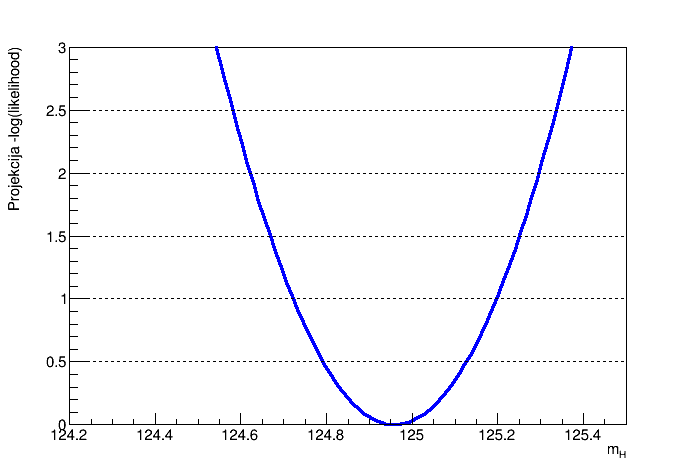
\includegraphics[width=0.9\textwidth]{test-23-8.png}
		 	\caption[Saturn viđen u ultraljubičastom svjetlu.]{\label{sl:sl8} Maximum likelihood za estimator srednje vrijednosti našeg modela prilagođenog na prave podatke }
		 \end{figure}
	 	Isprekidane linije na slici \ref{sl:sl8} predstavljaju 1, 2, 3, 4 i 5 $\sigma$ pogrešku. Tako nam 1 $\sigma$ pogreška na ovom grafu govori da ćemo s otprilike 68\% vjerojatnosti pronaći masu Higgsovog bozona u intervalu od 124,8 do 125,14 GeV. Vrijednost od 68\% smo dobili prema formuli \begin{equation}
	 	P=erf(\frac{n}{\sqrt{2}})
	 	\end{equation}, gdje je n u našem slučaju jednak 1.
		Isto tako možemo ustvrditi sa više od 99.999\% vjerojatnosti da Higgsov bozon ima masu u interavlu od 124,45 do 125,35 GeV.
		
		\subsection{Statističke i sistematske pogreške}
		Da bi znanstveno istraživanje imalo smisla potrebno ga je zaokružiti s posljednjim korakom, određivanjem statističkih i sistematskih pogreški.
		Statističku pogrešku možemo definirati kao neodređenost rezultata zbog konačne preciznosti uređaja i fluktuacija u uvjetima mjerenja. Takve pogreške se mogu smanjiti izradom preciznijih uređaja ili pak ponavljanjem broja mjerenja. Njih smo provodili kroz cijeli radi i direktno su ispisane na svakom grafu prilikom računanja parametara. Kao što im i sam naziv kaže može ih se izračunati statistički, eksplicitnom formulom. 
		
		
		Drugi tip pogrešaka su sistematske pogreške. One su rezultat pogreške čovjeka ili stroja prilikom mjerenja rezultata. Za razliku od statističkih pogrešaka, za ove vrste neodređenosti nema šablonizirane formule kojom je možemo izračunati. Takve pogreške znanstvenik procjenjuje osobno i stoga mogu biti pristrane. Npr. ako se pogreška zanemari može doći do krivog zaključka koji kasnije može imati fatalne posljedice. S druge strane ako je znanstvenik prekonzervativan može eksperiment proglasiti neuspjelim iako je bio na pragu velikog otkrića.
		U fizici visokih energija gdje se detektiraju na milijarde čestice i odvija na milijune reakcija bitan faktor je zamor materijala. Materija koja služi za detekciju čestica nastalih u sudarima međudjeluje s istima te mijenja svoj oblik i svojstva. Zato je bitno da znanstvenici uzimaju i takve promjene u obzir. Konstantno prilagođavanje na takve promjene te mijenjanje pojedinih vrijednosti direktno očitanih iz detektora je jedan od glavnih razloga uspješnosti takvih eksperimenata.
		Ipak u ovom radu mi ćemo sistematsku pogrešku mjerenja procjenjivati s gornjim i donjim statističkim granicama pojedinih parametara. Taj hibridan način računanja pogreške je dovoljno dobar za naše malo istraživanje, ali isto tako jasno je da moramo očekivati puno veću sistematsku pogrešku nego onu koju dobivaju znanstvenici u CERN-u.  
		
		\begin{figure}[H]
			\centering
			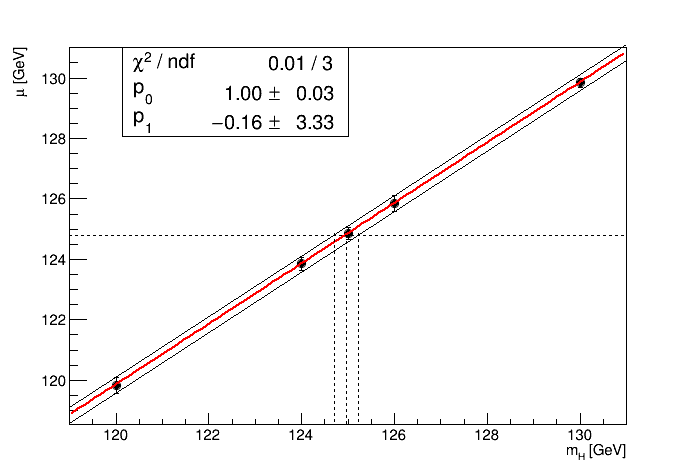
\includegraphics[width=0.9\textwidth]{sist-pogreska-fit-19-8.png}
			\caption[Procjena sistematske pogreške preko najveće gornje granice i najmanje donje granice statističke pogreške.]{\label{sl:sl9} Procjena sistematske pogreške preko najveće gornje granice i najmanje donje granice statističke pogreške.}
		\end{figure}
		
		Takav način procjene sistematske pogreške je zgodno i grafički prikazati (slike ~\ref{sl:sl9}). Odredili smo najveću gornju statističu pogrešku i najmanju donju statističku pogrešku parametara mase Higgsovog bozona, te povukli pravce kroz te točke paralelne na pravac koji se linearno prilagodio za različite vrijednosti mase Higgsovog bozona. Uvrštavajući m$_{\mathrm{H}}$ u izraz \begin{equation}
		\mu = p_0 \cdot m_H + p_1
		\end{equation}, dobili smo vrijednost $\mu$ te povukli konstantan pravac kroz tu vrijednost. Takav pravac je presjekao prethodno povučene pravce te smo izračunali lijevu i desnu sistematsku pogrešku na srednju vrijednost mase Higgsovog bozona.
		
	
	
		% Please add the following required packages to your document preamble:
		% \usepackage{multirow}
		\begin{table}[H]
			\centering
			\caption[Utjecaj pojedinog parametra na sistematsku pogrešku mase Higgsovog bozona]{\label{tab:sist-pogreske}Utjecaj pojedinog parametra na sistematsku pogrešku mase Higgsovog bozona}
			\begin{tabular}{?l|l|l|l?}
				\hlineRub
				Parametar                    & \makecell{Gornja i donja vrijednost \\ parametra} & \makecell{Gornja i donja vrijednost\\ mase Higgsovog bozona $m_{H}$} & Devijacija ($\sigma$) \\ \hline
				\multirow{2}{*}{$m_{H}$=124.96}     & $m_{HD}$=124.7                      &                           &        $\sigma_{D}$=0.26            \\
				& $m_{HG}$=125.23                      &                           &         $\sigma_{G}$=0.27           \\ \hline
				\multirow{2}{*}{$\mu$=1.00}     & $\mu_{D}$=0.89                      & $m_{H}$=124.97                          &     $\sigma_{D}$=0.01               \\
				& $\mu_{G}$=0.11                      & $m_{H}$=124.94                          &       $\sigma_{G}$=0.02             \\ \hline
				\multirow{2}{*}{$\sigma$=1.161} & $\sigma_{D}$=1.061                  & $m_{H}$=124.98                          &      $\sigma_{D}$=0.02              \\
				& $\sigma_{G}$=1.261                  & $m_{H}$=124.94                          &     $\sigma_{G}$=0.02               \\ \hline
				\multirow{2}{*}{$\alpha_{1}$=1.24} & $\alpha_{1D}$=1.04                  & $m_{H}$=124.99                          &       $\sigma_{D}$=0.03             \\
				& $\alpha_{1G}$=1.44                  & $m_{H}$=124.93                          &         $\sigma_{G}$=0.03           \\ \hline
				\multirow{2}{*}{$\alpha_{2}$=1.77} & $\alpha_{2D}$=1.36                  & $m_{H}$=124.95                          &      $\sigma_{D}$=0.01              \\
				& $\alpha_{2G}$=2.18                  & $m_{H}$=124.95                          &     $\sigma_{G}$=0.01               \\ \hline
				\multirow{2}{*}{$n_{1}$=2.035}    & $n_{1D}$=1.506                     & $m_{H}$=124.97                          &      $\sigma_{D}$=0.01              \\
				& $n_{1G}$=2.655                     & $m_{H}$=124.95                          &         $\sigma_{G}$=0.01           \\ \hline
				\multirow{2}{*}{$n_{2}$=3.192}    & $n_{2D}$=1.044                     & $m_{H}$=124.97                          &         $\sigma_{D}$=0.01           \\
				& $n_{2G}$=5.34                      & $m_{H}$=124.96                          &     $\sigma_{G}$=0               \\ \hline
				\multirow{2}{*}{$a$=-1.010}    & $a_{D}$=-1.59                      & $m_{H}$=125.01                          &        $\sigma_{D}$=0.05            \\
				& $a_{G}$=-0.43                      & $m_{H}$=124.97                          &        $\sigma_{G}$=0.01            \\ \hline
				\multirow{2}{*}{$b$=252}       & $b_{D}$=115                        & $m_{H}$=125.01                          &    $\sigma_{D}$=0.05                \\
				& $b_{G}$=389                        & $m_{H}$=124.96                          &      $\sigma_{G}$=0              \\ \hline
				\multirow{2}{*}{$c$=-14493}    & $c_{D}$=-22205                     & $m_{H}$=125.01                          &      $\sigma_{D}$=0.05              \\
				& $c_{G}$=-6731                      & $m_{H}$=124.96                          &        $\sigma_{G}$=0            \\ \hline
				\multirow{2}{*}{$coeff$=0.4}   & $coeff_{D}$=0.34                   & $m_{H}$=124.96                          &        $\sigma_{D}$=0            \\
				& $coeff_{G}$=0.46                   & $m_{H}$=124.96                          &     $\sigma_{G}$=0      \\
				\hline
				\multirow{1}{*}{$coeff$=0.4}   & $coeff_{D}$=0.34                   & $m_{H}$=124.96                          &        $\sigma_{D}$=0            \\
				& $coeff_{G}$=0.46                   & $m_{H}$=124.96                          &     $\sigma_{G}$=0      \\
				\hline
				\multicolumn{3}{r}{\multirow{2}{*}{TOTAL}}                                                                    & $\sigma_{D}$=0.28              \\
				\multicolumn{3}{r}{}                                                                                          & $\sigma_{G}$=0.27                  \\
				\hlineRub
		\end{tabular}
		\end{table}
	
		Kako smo radili i s drugim parametrima koji su davali određenu pogrešku, morali smo i njih uzeti u obzir. Program konačne prilagodbe funkcije na podatke smo izvrtili za sve pojedinačne parametre dok smo ostale držali fiksiranima i to smo ponovili za njihove donje i gornje granice. Konačno kvadratnom metodom smo sumirali sve gornje i donje pogreške. Jasno iz  tablice ~\ref{tab:sist-pogreske} da je najveći doprinos na ukupnu pogrešku imala pogreška srednje vrijednosti mase Higgsovog bozona, dok su ostale pogreške imale manji udio. 
	
		Konačno mjerenje nam daje za masu Higgsovog bozona
		m${_{\mathrm{H}}^{4\mu}}$ = 124,96 $\pm$ 0,17(stat.)$_{-0,28}^{+0,27}$(sist.) GeV = 124,96 $_{-0,33}^{+0,32}$ GeV.
		
		
		\subsection{Usporedba s rezultatima CMS-a i ATLAS-a}
		Za kraj, zanimljivo je usporediti naše rezultate sa onima nastalim u kolaboraciji tima znanstvenika iz CMS-a i ATLAS-a~\cite{kolaboracija}. U kanalu H$\rightarrow$ZZ$\rightarrow$4l dobivaju masu Higgsovog bozona 
		m${_{\mathrm{H}}^{4l}}$ = 125.15 $\pm$ 0,40 GeV
		= 125,15 $\pm$ 0,37 ( stat. ) $\pm$ 0,15 ( syst. ) GeV. Rasponi pogreške od srednje vrijednosti mase Higgsovog bozona se poklapaju sa našim rezultatima. Treba primjetiti da je naša statistička pogreška dosta manja, a razlog tome je što smo mi radili s većim brojem podataka. Isto tako naša sistematska pogreška je puno veća jer smo htjeli osigurati valjan rezultat, dok znanstvenici u CERN-u prilagođavaju gotovi svaki parametar koji nad sobom doživljava promjene svakim novim sudarom u detektoru. 
		 
		
		
		\begin{figure}[H]
						
			\centering
			\begin{subfigure}[b]{0.49\textwidth}
				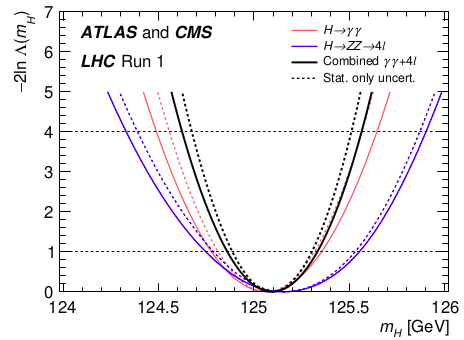
\includegraphics[width=\textwidth]{usporedba1.png}
				\caption{}
				\label{sl:sl91}
			\end{subfigure}	
			~ %add desired spacing between images, e. g. ~, \quad, \qquad, \hfill etc. 
			%(or a blank line to force the subfigure onto a new line)
		\begin{subfigure}[b]{0.49\textwidth}
			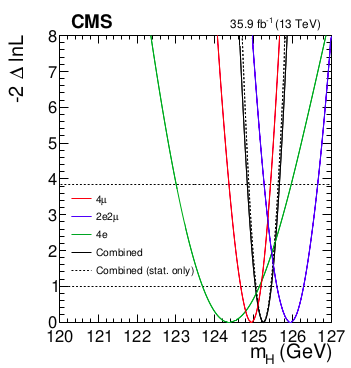
\includegraphics[width=\textwidth]{usporedba2.png}
			\caption{}
			\label{sl:sl10} 
		\end{subfigure}
			
			~ %add desired spacing between images, e. g. ~, \quad, \qquad, \hfill etc. 
			%(or a blank line to force the subfigure onto a new line)
			\caption{a) Negativne loglikelihood funkcije mase Higgsovog bozona za različite kanale preuzete iz ~\cite{kolaboracija}	b)Negativne loglikelihood funkcije mase Higgsovog bozona za različite kanale preuzete iz ~\cite{cms-clanak} }\label{fig:grafovi-978}
		\end{figure}		
		
		
		U radu ~\cite{cms-clanak} kanal H$\rightarrow$ZZ$\rightarrow$4l je raščlanjen na kanale H$\rightarrow$ZZ$\rightarrow$4$\mu$, H$\rightarrow$ZZ$\rightarrow$4e i H$\rightarrow$ZZ$\rightarrow$2e2$\mu$.
		Konačna masa u kanalu H$\rightarrow$ZZ$\rightarrow$4$\mu$ bila je 
		m${_{\mathrm{H}}^{4\mu}}$ = 124,94 $\pm$ 0,25 (stat.) $\pm$ 0,08 (syst.) GeV. I za ovaj rad možemo donijeti iste zaključke u usporedbi sa našim rezultatima.
		
		\newpage
		\section{Zaključak}
		Prema teoriji SM-a konstruirali smo double Crystal ball funkciju, koja se u konačnici pokazala jako dobro prilikom uspoređivanja s pravim podatcima. Konačni dobiveni rezultat za masu Higgsovog bozona je 
		m${_{\mathrm{H}}^{4\mu}}$ = 124,96 $\pm$ 0,17(stat.)$_{-0,28}^{+0,27}$(sist.) GeV, a usporedbom tog rezultata s onima iz CERN-a vidimo slaganje unutar pogreške. Zbog većeg broja podataka statistička pogreška je bila manje nego u CERN-u, ali je sistematska bila puno veća što je bilo za i očekivati. Iako je ovaj rad pokazao jako dobre rezultate, ima još dosta mjesta za napredak ponajviše u segmentu određivanja sistematske pogreške. Također bilo bi interesantno promatrati i ostale kanale nastajanja i raspadanja Higgsovog bozona te koliki bi bio njihov utjecaj da ih uključimo u analizu. 
		U vrijeme pisanja ovog rada, znanstvenici u CERN-u rade na istim podatcima te će biti jako zanimljivo usporediti njihove rezultate s našim sadašnjim. Statističku pogrešku očekujemo da bude otprilike jednaka, dok za sistematsku pogrešku očekujemo jako niske vrijednosti. Također, u svibnju 2021. godine očekuje se pokretanje 3. generacije prikupljanja podataka u LHC-u koje će trajati do 2024. godine, kada će se opet ugasiti na 3 godine. Predviđanja su da će se uspijeti skupiti 2 puta više podataka nego u periodu od 2009. do 2018. godine. Razvitkom tehnologije, koja ponajviše omogućuje jako brzo obradu ogromnog broja podataka, 2027.godine predviđa se cjeloukpuna nadogradnja LHC-a u Veliki hadronski ubrzivač visokog luminoziteta (eng. High luminosity LHC) od kojeg se očekuje čak 10 puta više prikupljenih podataka.\\
		 Iako se dosadašnji rezultati čine kao kraj nekakavog istraživanja i zatvaranje poglavlja, ovo je samo početak za sve što nam slijedi! 
		
		
		\stepcounter{section} %NE brisati (broji Literaturu kao novo poglavlje)
		% UNIJETI LITERATURU NAREDBAMA \bibitem UNUTAR thebibliography
		\newpage
		{\raggedright
			\begin{thebibliography}{99}
						
				
				\bibitem{uvod}
				J. Allday, \textit{Quarks, Leptons and the Big Bang: Second edition},CRC Press, Philadelphia 2002.
				
				\bibitem{standardni_model}
				Wikipedija, Standardni model, URL: \url{https://hr.wikipedia.org/wiki/Standardni_model} (25.8.2020.)
				
				\bibitem{uvod2}
				 S. Veselinović, \textit{Elementarne čestice}, završni rad, Sveučilište Josipa Jurja Strossmayera u Osijeku, Osijek 2014.
				 
				 \bibitem{uvod3}
				 Wikipedia, Foton, URL: \url{https://hr.wikipedia.org/wiki/Foton} (2. 6. 2020.).
				 
				 
				 
				 \bibitem{uvod4}
				 Wikipedia, Bozoni, URL: \url{https://hr.wikipedia.org/wiki/Bozoni} (2. 6. 2020.).
				 
				 
				 \bibitem{uvod5}
				 				 Wikipedia, Gluon, URL: \url{https://hr.wikipedia.org/wiki/Gluon} (2. 6. 2020.).
				 
				
				\bibitem{doktorat}
				T. Šćulac, \textit{Measurements of Higgs boson properties
					in the four-lepton channel in pp collisions
					at centre-of-mass energy of 13 TeV with
					the CMS detector}, Palaiseau, France, 2018.
				
				\bibitem{dokt2}
				D. Zanzi, \textit{Search for the Standard Model Higgs boson produced in
				association with a pair of top quarks and decaying into
				channel at $\sqrt{s}$ = 8 TeV
				with the ATLAS experiment at the LHC}, Faculty of science University of Copenhagen, 2011.
							
				\bibitem{rokoplestina}
				R. Pleština, \textit{Potencijal CMS detektora za
				potragu za Higgsovim bozonom kroz
				kanal raspada \begin{math}
				H \rightarrow ZZ^{*} \rightarrow 4e^{\pm}
				\end{math}}, Sveučilište u Zagrebu, 2008.
				
				\bibitem{cernweb}
				CERN, Higgs boson, URL: \url{https://home.cern/science/physics/higgs-boson}(22. 8. 2020.).
				
				
				\bibitem{cern-wiki}
				Wikipedia, CERN, URL: \url{https://en.wikipedia.org/wiki/CERN}(17. 8. 2020.).
				
				
				\bibitem{cern-lhc}
				CERN, LHC, URL: \url{https://home.cern/science/accelerators/large-hadron-collider}(22. 8. 2020.).
				
				\bibitem{cern-slika}
				S. Ruth, S. Davis, \textit{Interactive Slice of the CMS detector}, CMS-OUTREACH-2016-027, (3. 8. 2016.) 
				
				
				\bibitem{cern-sustav tragova}
				CMS, Tracking, URL: \url{http://cms.cern/detector/identifying-tracks}(22. 8. 2020.).
				
				
				\bibitem{mc-simulacije}
				Wikipedia, Monte Carlo method, URL: \url{https://en.wikipedia.org/wiki/Monte_Carlo_method} (17. 8. 2020.).
				
				
				\bibitem{royal-sm}
				T. Shears, \textit{The Standard Model}, Phil. Trans. R. Soc. A 370, 805–817, 2012.
				
				\bibitem{royal-sm8}
				T. Shears, \textit{The Standard Model}, Phil. Trans. R. Soc. A 370, 813, 2012.
				
				\bibitem{royal-sm9}
				T. Shears, \textit{The Standard Model}, Phil. Trans. R. Soc. A 370, 814, 2012.
				
				\bibitem{roofit}
				Wikipedia, ROOT, URL: \url{https://en.wikipedia.org/wiki/ROOT}(17. 8. 2020.).
				
				
				\bibitem{pileup}
				QUANTUM DIARIES, URL: \url{https://www.quantumdiaries.org/2011/10/25/piling-up/} (2011.).
				
				
				\bibitem{geant4}
				CERN, GEANT4, URL: \url{https://geant4.web.cern.ch/}(22. 8. 2020.).
				

					\bibitem{pdf}
				C. Forbes i dr. \textit{Statistical Distributions}, Wiley(4. izdanje), New Jersey, 2010.
				
				\bibitem{87}
				P. Nason. \textit{A New method for combining NLO QCD with shower Monte Carlo
				algorithms}, JHEP, 11:040, 2004.
				
				\bibitem{88}
				S. Frixione i dr. \textit{Matching NLO QCD computations with Parton Shower simula-
				tions: the POWHEG method}, JHEP, 11:070, 2007.
				
				\bibitem{89}
				S. Alioli i dr. \textit{NLO vector-boson production matched with shower in POWHEG},
				JHEP, 07:060, 2008.
				
				\bibitem{93}
				Y. Gao i dr. \textit{Spin determination of single-produced resonances at hadron colliders}, Phys. Rev., D81:075022, 2010.
				
				\bibitem{94}
				S. Bolognesi i dr. \textit{On the spin and parity of a single-produced resonance at the
				LHC}, Phys. Rev., D86:095031, 2012.
				
				\bibitem{95}
				I. Anderson i dr. \textit{Constraining anomalous HVV interactions at proton and lepton
				colliders}, Phys. Rev., D89(3):035007, 2014.
				
				\bibitem{96}
				A. Gritsan i dr. \textit{Constraining anomalous Higgs boson couplings to the heavy
				flavor fermions using matrix element techniques} Phys. Rev., D94(5):055023,
				2016.
				
				\bibitem{cms-pileup}
				CERN, HOW CMS WEEDS OUT PARTICLES THAT PILE UP, URL: \url{https://cms.cern/news/how-cms-weeds-out-particles-pile}(22. 8. 2020.).
				
				
				\bibitem{rooaddpdf}
				ROOT, RooFit, RooAddPdf, URL: \url{https://root.cern.ch/doc/master/classRooAddPdf.html}(22. 8. 2020.).
				
				
				\bibitem{kolaboracija}
				CMS Collaboration, Physics Letters B \textbf{716} 30–61, \textit{Observation of a new boson at a mass of 125 GeV with the CMS experiment at
					the LHC}, 2012.
				
				\bibitem{cms-clanak}
				CMS Collaboration,Journal of High Energy Physics A \textbf{47},  \textit{Measurements of properties of the Higgs boson decaying
					into the four-lepton final state in pp collisions at
					$\sqrt{s}$ = 13 TeV}, 2017.
				
				
				\bibitem{atlas-rad}
				The ATLAS and CMS Collaborations, Phys. Rev. Lett. \textbf{114} 191803,  \textit{Combined Measurement
					of the Higgs Boson Mass in pp
					Collisions at $\sqrt{s}$ = 7 and 8 TeV with the ATLAS and CMS
					Experiments}, 2015.
				
				
			\end{thebibliography}
		}
		
		% IZBRISATI DODATKE (appendix) AKO NE POSTOJE
		\newpage \appendix
		\section{Osnovne funkcije i implementacija RooFit biblioteke u  C++}
		Za rad u ROOT-u i RooFit-u potrebno je uvesti biblioteke u C++ program. Neke od najvažnijih su:
		\begin{minted}[linenos,tabsize=0,breaklines]{cpp}
		#include <TROOT.h>
		#include <TChain.h>
		#include <TFile.h>
		#include "RooRealVar.h"
		#include "RooConstVar.h"
		#include "RooAddPdf.h"
		#include "RooDataSet.h"
		#include "RooGenericPdf.h"
		#include "RooPlot.h"
		\end{minted}
		
		Za razliku od standardnog inicijaliziranja varijabli u C++, RooFit je objektno-orjentirana biblioteka sa vlastitim klasama i zahtjeva da se sve obavlja preko objekata tih klasa.
		RooRealVar predstavlja numeričku varijablu. Postoji više različitih konstruktora koji inicijaliziraju RooRealVar ovisno o broju prosljeđenih parametara.
		\begin{minted}[linenos,tabsize=0,breaklines]{cpp}
		RooRealVar mean("mean","Mean of Gaussian",125,105.0,140.0) ; //(ime, naslov, vrijednost, min_vrijednost, max_vrijednost)
		RooRealVar sigma("sigma","Width of Gaussian",0.1,5.0) ; //(ime, naslov, min_vrijednost, max_vrijednost)
		\end{minted}
		
		RooFit je jako razvijena biblioteka i nije čudno što su neke osnovne funkcije već implementirane. Jedna od takvih je i Gaussian. Ako želimo naše podatke prilagoditi na Gaussovu krivulju moramo uključiti biblioteku te koristimo iduću naredbu:
		\begin{minted}[linenos,tabsize=0,breaklines]{cpp}
		#include "RooGaussian.h"
		//.......................
		RooGaussian gauss("gauss","gauss(x,mean,sigma)",x,mean,sigma) ; 
		\end{minted}
		
		Često nam osnovne funkcije nisu dovoljne, već moramo sami konstruirati funkciju na koju želimo prilagoditi podatke. Primjer kvadratne funkcije:
		
		\begin{minted}[linenos,tabsize=0,breaklines]{cpp}
		#include "RooGenericPdf.h"
		.........................
		RooRealVar  x("x","x",105,140) ;
		RooRealVar a("a","a",-1,-5,5) ;
		RooRealVar b("b","b",250,-50,450) ;
		RooRealVar c("c","c",-15000,-20000,10000) ;
		RooGenericPdf backg("backg","a*x*x + b*x + c", RooArgSet(x,a,b,c));
		\end{minted}
		
		Nakon što smo odredili funkciju po kojoj prilagođavmo podatke i njene parametre, idući korak je generiranje podataka. Podatke možemo učitati iz neke datoteke ili pak generirati "toy" podatke koji će savršeno pratiti našu funkciju:
		
		\begin{minted}[linenos,tabsize=0,breaklines]{cpp}
		RooDataSet *data("data","dataset with ZZMass",fChain,ZZMass) ; //učitavanje iz fChain-a
		RooDataSet *data = gauss.generate(x,1000) ; //generiranje 1000 toy podataka po Gauss-u
		\end{minted}
		
		
		
		Kao što već znamo, osnovna funkcionalnost RooFit-a je prilagođavanje funkcije na podatke, a to radimo idućom naredbom:
		
		\begin{minted}[linenos,tabsize=0,breaklines]{cpp}
		gauss.fitTo(data);
		\end{minted}
		
		Nakon numeričkog izvršavanja prilagodbe funkcije na podatke, bitno je to i grafički prikazati:
		
		\begin{minted}[linenos,tabsize=0,breaklines]{cpp}
		#include "RooPlot.h"
		....................
		RooPlot* mesframe = x.frame();
		data->plotOn(mesframe); //prikazuje podatke kao točkice na grafu
		gauss.plotOn(mesframe, LineColor(kRed)); //prikazuje prilagodbe funkcijenu Gaussovu krivulju crvene boje
		gauss.paramOn(mesframe, Layout(0.7)); //prikazuje parametre i statističke pogreške istih na platnu 
		mesframe->SetXTitle("Oznaka na osi X");
		mesframe->SetYTitle("Oznaka na osi Y");
		mesframe->SetTitle("Naslov grafa");
		mesframe->Draw();
		\end{minted}
		
		Često ne prilagođavamo podatke na samo jednu funkciju, nego na model koji se sastoji od više njih:
		
		\begin{minted}[linenos,tabsize=0,breaklines]{cpp}
		#include "RooAddPdf.h"
		......................
		RooRealVar ngauss("nsig","#gauss events",84.30866); //predstavlja integral funkcije nakon prilagodbe funkcije
		RooRealVar nbkg("nbkg","#nbkg events",128.789);
		RooAddPdf model("model","s+b",RooArgList(gauss,backg),RooArgList(ngauss,nbkg));
		model.fitTo(*data);
		\end{minted}
		
		\subsection{Kompleksnije funkcionalosti}
		Dodavanje težine događajima je bitan proces kod simulacija, jer možemo izgenerirati puno više događaja nego u pravom eksperimentu, ali zato svakom događaju moramo dodati određenu vjerojatnost zbivanja(težina).
		\begin{minted}[linenos,tabsize=0,breaklines]{cpp}
		#include "RooFormulaVar.h"
		..........................
		RooRealVar  x("x","x",105,140) ;
		RooRealVar  a("a","a",1,0.1,2.1) ;
		RooRealVar  b("b","b",125,140,160) ;
		RooRealVar  c("c","c",1500,-200,6250) ;
		RooDataSet test("test","test", RooArgSet(x));
		RooFormulaVar wFunc("gen","a*(b+c)",RooArgSet(a,b,c)) ;
		//alternativni načina zapisa za RooFormulaVar:
		//RooFormulaVar wFunc("gen","@0*(@1 + @2)",RooArgList(a,b,c));
		RooRealVar* w = (RooRealVar*) test.addColumn(wFunc) ;
		RooDataSet wdata(test.GetName(),test.GetTitle(),&test, *test.get(),0,w->GetName()) ;
		gauss.fitTo(wdata);
		\end{minted}
		
		
		Također, možemo konstruirati loglikelihood i profile likelihood funkciju za određeni parametar (u primjeru ispod, mean):
		
		\begin{minted}[linenos,tabsize=0,breaklines]{cpp}
		#include "RooAbsReal.h"
		#include "RooMinimizer.h"
		#include <TCanvas.h>
		.........................
		RooAbsReal* nll = model.createNLL(*data, NumCPU(4));
		RooMinimizer(*nll).migrad();
		RooPlot* frame1 = mean.frame(Bins(100),Range(120.5,130.5),Title("LL and profileLL in frac")) ;
		nll->plotOn(frame1,ShiftToZero()) ;
		RooAbsReal* pll_frac = nll->createProfile(mean) ;
		pll_frac->plotOn(frame1,LineColor(kRed)) ;
		frame1->SetMinimum(0);
		frame1->SetMaximum(5);
		TCanvas *canv = new TCanvas("rf605_profilell","rf605_profilell",800, 400);
		canv->cd(1) ; frame1->GetYaxis()->SetTitleOffset(1.4) ; frame1->Draw() ;
		canv->SaveAs("model-maxlikelihood.png");
		delete pll_frac ;
		delete nll ;*
		\end{minted}
		
		
	
		
	\end{linenumbers}
\end{document}
